% Options for packages loaded elsewhere
\PassOptionsToPackage{unicode}{hyperref}
\PassOptionsToPackage{hyphens}{url}
\documentclass[
  11pt,
]{article}
\usepackage{xcolor}
\usepackage[margin=1in]{geometry}
\usepackage{amsmath,amssymb}
\setcounter{secnumdepth}{-\maxdimen} % remove section numbering
\usepackage{iftex}
\ifPDFTeX
  \usepackage[T1]{fontenc}
  \usepackage[utf8]{inputenc}
  \usepackage{textcomp} % provide euro and other symbols
\else % if luatex or xetex
  \usepackage{unicode-math} % this also loads fontspec
  \defaultfontfeatures{Scale=MatchLowercase}
  \defaultfontfeatures[\rmfamily]{Ligatures=TeX,Scale=1}
\fi
\usepackage{lmodern}
\ifPDFTeX\else
  % xetex/luatex font selection
\fi
% Use upquote if available, for straight quotes in verbatim environments
\IfFileExists{upquote.sty}{\usepackage{upquote}}{}
\IfFileExists{microtype.sty}{% use microtype if available
  \usepackage[]{microtype}
  \UseMicrotypeSet[protrusion]{basicmath} % disable protrusion for tt fonts
}{}
\makeatletter
\@ifundefined{KOMAClassName}{% if non-KOMA class
  \IfFileExists{parskip.sty}{%
    \usepackage{parskip}
  }{% else
    \setlength{\parindent}{0pt}
    \setlength{\parskip}{6pt plus 2pt minus 1pt}}
}{% if KOMA class
  \KOMAoptions{parskip=half}}
\makeatother
\usepackage{longtable,booktabs,array}
\usepackage{caption}
\captionsetup[table]{skip=6pt}
\newcounter{none} % for unnumbered tables
\usepackage{calc} % for calculating minipage widths
% Correct order of tables after \paragraph or \subparagraph
\usepackage{etoolbox}
\makeatletter
\patchcmd\longtable{\par}{\if@noskipsec\mbox{}\fi\par}{}{}
\makeatother
% Allow footnotes in longtable head/foot
\IfFileExists{footnotehyper.sty}{\usepackage{footnotehyper}}{\usepackage{footnote}}
\makesavenoteenv{longtable}
\usepackage{graphicx}
\makeatletter
\newsavebox\pandoc@box
\newcommand*\pandocbounded[1]{% scales image to fit in text height/width
  \sbox\pandoc@box{#1}%
  \Gscale@div\@tempa{\textheight}{\dimexpr\ht\pandoc@box+\dp\pandoc@box\relax}%
  \Gscale@div\@tempb{\linewidth}{\wd\pandoc@box}%
  \ifdim\@tempb\p@<\@tempa\p@\let\@tempa\@tempb\fi% select the smaller of both
  \ifdim\@tempa\p@<\p@\scalebox{\@tempa}{\usebox\pandoc@box}%
  \else\usebox{\pandoc@box}%
  \fi%
}
% Set default figure placement to htbp
\def\fps@figure{htbp}
\makeatother
% definitions for citeproc citations
\NewDocumentCommand\citeproctext{}{}
\NewDocumentCommand\citeproc{mm}{%
  \begingroup\def\citeproctext{#2}\cite{#1}\endgroup}
\makeatletter
 % allow citations to break across lines
 \let\@cite@ofmt\@firstofone
 % avoid brackets around text for \cite:
 \def\@biblabel#1{}
 \def\@cite#1#2{{#1\if@tempswa , #2\fi}}
\makeatother
\newlength{\cslhangindent}
\setlength{\cslhangindent}{1.5em}
\newlength{\csllabelwidth}
\setlength{\csllabelwidth}{3em}
\newenvironment{CSLReferences}[2] % #1 hanging-indent, #2 entry-spacing
 {\begin{list}{}{%
  \setlength{\itemindent}{0pt}
  \setlength{\leftmargin}{0pt}
  \setlength{\parsep}{0pt}
  % turn on hanging indent if param 1 is 1
  \ifodd #1
   \setlength{\leftmargin}{\cslhangindent}
   \setlength{\itemindent}{-1\cslhangindent}
  \fi
  % set entry spacing
  \setlength{\itemsep}{#2\baselineskip}}}
 {\end{list}}
\usepackage{calc}
\newcommand{\CSLBlock}[1]{\hfill\break\parbox[t]{\linewidth}{\strut\ignorespaces#1\strut}}
\newcommand{\CSLLeftMargin}[1]{\parbox[t]{\csllabelwidth}{\strut#1\strut}}
\newcommand{\CSLRightInline}[1]{\parbox[t]{\linewidth - \csllabelwidth}{\strut#1\strut}}
\newcommand{\CSLIndent}[1]{\hspace{\cslhangindent}#1}
\setlength{\emergencystretch}{3em} % prevent overfull lines
\providecommand{\tightlist}{%
  \setlength{\itemsep}{0pt}\setlength{\parskip}{0pt}}
\usepackage{caption}
\captionsetup[figure]{labelformat=empty}
\captionsetup[table]{labelformat=empty}
\usepackage{bookmark}
\IfFileExists{xurl.sty}{\usepackage{xurl}}{} % add URL line breaks if available
\urlstyle{same}
% fallback for those not using the hyperref driver hyperxmp:
\makeatletter
\@ifundefined{xmpquote}{\newcommand{\xmpquote}[1]{#1}}{}
\makeatother
\hypersetup{
  pdftitle={Same Job{,} Different Technology? Renewable--Nonrenewable Wage Gaps Within Occupations in U.S. Power Generation Establishments{,} 2021--2025},
  pdfauthor={{[}Author name and affiliation{]}},
  hidelinks,
  pdfcreator={LaTeX via pandoc}}

\title{Same Job, Different Technology? Renewable--Nonrenewable Wage Gaps
Within Occupations in U.S. Power Generation Establishments, 2021--2025}
\author{{[}Author name and affiliation{]}}
\date{September 2026}

\begin{document}
\maketitle

\subsection{Abstract}\label{abstract}

Renewable generation employment in the United States expanded rapidly in
the early 2020s, but whether the new jobs pay like the fossil-fuel and
nuclear jobs they partly replace remains unclear, because most evidence
on ``green'' pay compares occupations rather than employers. This study
asks how much less, or more, renewable generation establishments pay
workers in the same detailed occupation, how the gap differs across
technologies and occupational classes, and whether it changed between
2021 and 2025. Using the Bureau of Labor Statistics Occupational
Employment and Wage Statistics for 2021--2025, I analyze 1,877
industry-by-occupation-by-year cells covering in-house employees of
private electric power generation establishments, estimating
employment-weighted regressions with occupation-by-year fixed effects,
wild cluster bootstrap inference, and a Kitagawa decomposition. Within
the same occupation and year, renewable establishments paid 11.5\% less
than fossil-fuel and nuclear establishments. The gap was concentrated in
solar (−12.1\%), wind (−7.3\%), and biomass and geothermal (−24.4\%)
generation, whereas hydroelectric pay was statistically
indistinguishable from fossil-fuel pay and nuclear paid 11.6\% more. The
gap was three times larger for blue-collar trades (−16.4\%) than for
professional and managerial occupations (−5.5\%). Comparing estimates
built from non-overlapping survey panels, the gap did not narrow while
renewable employment doubled, and the worker-weighted gap widened as
newly shared occupations entered. Renewable expansion has so far
reproduced, not closed, a pay penalty that falls hardest on manual
workers, the group at the center of just-transition debates.

\textbf{Keywords:} energy transition; just transition; renewable energy;
wage inequality; occupations; job quality

\textbf{Highlights}

\begin{itemize}
\tightlist
\item
  Renewable plants pay 11.5\% less than fossil and nuclear plants for
  the same occupation.
\item
  Solar, wind, and biomass pay less; hydro matches fossil; nuclear pays
  11.6\% more.
\item
  The renewable pay gap is three times larger for blue-collar trades
  than for managers.
\item
  The within-occupation gap did not narrow from 2021 to 2025 as
  renewable jobs doubled.
\item
  Pay penalties at the 10th percentile (−20\%) exceed those at the 90th
  (−6\%).
\end{itemize}

\subsection{1. Introduction}\label{introduction}

Electricity generation is where the U.S. energy transition is most
visible in the labor market. Between the May 2021 and May 2025 rounds of
the federal establishment wage survey used in this study, employment in
private renewable generation establishments roughly doubled, from about
18,000 to 36,000 workers in published occupation cells, while employment
in fossil-fuel and nuclear generation was flat at about
107,000--110,000. The same years saw new federal tax credits for clean
electricity under the 2022 Inflation Reduction Act. For workers, the
question that matters is not only how many renewable jobs exist but what
they pay. A transition that moves electricians, mechanics, and operators
from coal and gas plants into solar and wind plants at lower pay would
redistribute the costs of decarbonization onto the workers it was meant
to protect, which is the central concern of the just-transition agenda
{[}\citeproc{ref-stevis2015global}{1},\citeproc{ref-mccauley2018just}{2}{]}.

Existing evidence conflicts, largely because studies measure different
things. Occupation-based analyses find that green and renewable jobs sit
in occupations that pay more than average
{[}\citeproc{ref-vona2019measures}{3},\citeproc{ref-curtis2023green}{4}{]},
while employer-based studies find that clean-energy firms pay no more
than legacy energy firms once education is held constant
{[}\citeproc{ref-colmer2025nice}{5}{]}. Neither answers the question a
displaced fossil-fuel worker faces: will I be paid the same for the same
job at a renewable plant?

This article answers that question directly. I use the Bureau of Labor
Statistics (BLS) Occupational Employment and Wage Statistics (OEWS),
which publish employment and mean wages for each detailed occupation
separately in each of eight electric power generation industries defined
by technology. Comparing the same detailed occupation across
technologies within the same survey round separates differences in pay
for a given classified job from differences in occupational mix. Five
annual rounds, May 2021 through May 2025, allow me to ask whether any
gap changed during the period of rapid renewable growth. Because each
OEWS round pools three years of survey panels, I test change using
rounds that share no panels.

Drawing on research on interindustry and between-workplace pay
differences
{[}\citeproc{ref-krueger1988efficiency}{6},\citeproc{ref-card2013workplace}{7}{]}
and on relational and durable-inequality accounts of how organizations
allocate rewards
{[}\citeproc{ref-tilly1998durable}{8},\citeproc{ref-tomaskovicdevey2019relational}{9}{]},
I argue that generation technologies are also organizational contexts
with different pay-setting institutions. That argument predicts a
within-occupation renewable penalty concentrated in newer technologies
and in blue-collar occupations, and it predicts that the penalty
persists despite growth. An ecological-modernization view
{[}\citeproc{ref-spaargaren1992sociology}{10}{]} instead predicts that
growth and subsidies would narrow it.

The results largely support the institutional account. Renewable
establishments paid about 11.5\% less than nonrenewable establishments
for the same occupation, the gap was concentrated in the newer
technologies and in blue-collar trades, and it did not narrow between
rounds that share no survey panels. The article contributes to energy
social science a technology-specific, occupation-matched benchmark of
renewable job quality during the early 2020s build-out, and it shows
that the renewable label hides the variation that matters for workers.
Section 2 develops the argument and hypotheses, Section 3 describes the
data and methods, Section 4 presents results, and Sections 5 and 6
discuss implications and limitations.

\subsection{2. Background and theory}\label{background-and-theory}

\subsubsection{2.1 Good jobs in the energy
transition?}\label{good-jobs-in-the-energy-transition}

In 2023, clean-energy employment in the United States grew more than
twice as fast as the rest of the energy sector and the economy, and
electric power generation is one of its main sites
{[}\citeproc{ref-doe2024useer}{11}{]}. Whether this amounts to a just
transition depends on more than job counts. The just-transition idea
originated in the labor movement as a demand that workers not bear the
costs of environmental policy
{[}\citeproc{ref-stevis2015global}{1},\citeproc{ref-ilo2014just}{12}{]},
and energy-justice scholars extended it into a broader principle for
sharing the burdens and benefits of decarbonization
{[}\citeproc{ref-mccauley2018just}{2},\citeproc{ref-newell2013political}{13},\citeproc{ref-healy2017politicizing}{14}{]}.
Reviews call for closer attention to what the shift away from fossil
fuels means for workers and their communities
{[}\citeproc{ref-beckfield2023social}{15},\citeproc{ref-carley2020justice}{16}{]},
many of which are highly exposed
{[}\citeproc{ref-raimi2022mapping}{17}{]}. Interviews with unionized
energy workers show that their expectations of the transition depend on
whether their skills fit renewable industries and whether conditions
there would strengthen or weaken their bargaining power
{[}\citeproc{ref-sicotte2022necessary}{18}{]}. Because pay is a core
component of job quality {[}\citeproc{ref-kalleberg2011good}{19}{]}, the
question is whether the jobs renewable energy creates pay like the ones
they partly replace.

\subsubsection{2.2 What we know about green and renewable
wages}\label{what-we-know-about-green-and-renewable-wages}

Evidence on green wages is inconsistent, partly because studies compare
different quantities. A task-based measure for U.S. local labor markets
finds that green employment carried a wage premium of about four percent
{[}\citeproc{ref-vona2019measures}{3}{]}, and green jobs in Japan pay
more mainly because of their task content
{[}\citeproc{ref-kuai2025estimating}{20}{]}. Using online job postings,
{[}\citeproc{ref-curtis2023green}{4}{]} estimate that solar and wind
openings cluster in occupations whose average pay is roughly a fifth
above the national mean. Their measure, however, gives each posting the
economy-wide average wage of its occupation: it captures the
occupational mix of renewable hiring, not what renewable employers pay
for a given job. Studies that observe employers are less optimistic.
Linked employer-employee records indicate that clean-energy firms pay no
more than legacy energy firms once education is held constant, and that
few workers move from legacy to clean employers
{[}\citeproc{ref-colmer2025nice}{5}{]}; transitions from
carbon-intensive into green jobs absorb under one percent of those
leaving carbon-intensive work
{[}\citeproc{ref-curtis2024workers}{21}{]}. Norwegian evidence points to
a green-firm premium below the premium paid in high-carbon industries
{[}\citeproc{ref-godoy2025green}{22}{]}, and industry reports show solar
near the bottom of median wages across energy technologies
{[}\citeproc{ref-lehmann2020wages}{23}{]}. Reviews note inconsistent
definitions and comparison groups and a focus on job numbers rather than
pay
{[}\citeproc{ref-bradley2025empirical}{24}--\citeproc{ref-pearse2022labour}{26}{]}.

These studies leave a specific gap. Occupation-level measures cannot say
whether an electrician at a solar plant earns what an electrician at a
gas plant earns, and firm-level studies group heterogeneous technologies
into a single ``clean'' category. I know of no study that holds detailed
occupation constant while comparing pay across generation technologies,
or that asks whether such a gap narrowed as renewable generation
employment expanded rapidly in the early 2020s.

\subsubsection{2.3 Why the same job pays differently across
sectors}\label{why-the-same-job-pays-differently-across-sectors}

Where people work matters for pay, independent of what they do. Industry
wage differentials persist when worker skill, job conditions, and
employer size are held constant, a pattern
{[}\citeproc{ref-krueger1988efficiency}{6}{]} interpret as evidence that
high-wage industries pay above market-clearing rates. Employer effects
account for a substantial share of wage variation
{[}\citeproc{ref-abowd1999high}{27}{]}, and growing pay differences
between workplaces account for a large share of the rise in earnings
inequality in Germany {[}\citeproc{ref-card2013workplace}{7}{]} and the
United States
{[}\citeproc{ref-barth2016where}{28}--\citeproc{ref-tomaskovicdevey2020rising}{30}{]}.
Sociologists interpret these patterns relationally: organizations
distribute rewards through claims-making shaped by workers' bargaining
position, organizational resources, and institutional history
{[}\citeproc{ref-tomaskovicdevey2019relational}{9},\citeproc{ref-wilmers2021consolidated}{31}{]},
and categorical distinctions become durable when they are built into
organizational routines {[}\citeproc{ref-tilly1998durable}{8}{]}.
Licensing and unionization raise pay for those inside the boundary
{[}\citeproc{ref-weeden2002why}{32}{]}, and unions have historically
compressed wages and upheld pay norms
{[}\citeproc{ref-western2011unions}{33},\citeproc{ref-rosenfeld2014unions}{34}{]}.
Much of the gender wage gap likewise reflects sorting across occupations
and establishments rather than unequal pay within the same job
{[}\citeproc{ref-petersen1995separate}{35},\citeproc{ref-cohen2003individuals}{36}{]}.

Applied to power generation, this literature suggests treating
technology as an organizational context as well as an engineering
choice. {[}\citeproc{ref-winner1980artifacts}{37}{]} argued, with
nuclear and solar power as examples, that technologies can be bound up
with particular arrangements of authority and organization. I conjecture
that a similar logic applies to employment relations. Fossil-fuel and
nuclear plants are large, capital-intensive, long-lived facilities, many
built under the regulated-utility model with internal labor markets and
formal job ladders; wind and solar generation is newer and more modular,
with small permanent operations workforces. Union and project-labor
coverage in 2023 was 16 to 19 percent in coal, natural gas, and nuclear
generation, compared with 11 to 14 percent in solar and wind and 13
percent in water power {[}\citeproc{ref-doe2024useer}{11}{]}. If
pay-setting institutions link sector to wages, I expect that, within the
same detailed occupation, renewable generation establishments pay lower
mean wages than nonrenewable establishments (H1). Because renewable
hiring is concentrated in occupations that pay well on average
{[}\citeproc{ref-curtis2023green}{4}{]}, I also expect that occupational
composition does not account for the renewable disadvantage, so the
within-occupation gap is at least as large as the raw gap (H5).

\subsubsection{2.4 Technologies, occupations, and
time}\label{technologies-occupations-and-time}

The same argument implies heterogeneity. If the gap reflects the
organizational form of newer technologies rather than renewable energy
as such, it should be concentrated in solar, wind, biomass, and
geothermal generation, negligible for hydroelectric generation, whose
plants long predate the recent build-out, and absent or reversed for
nuclear generation, the most institutionally consolidated technology
(H2). Institutional protections also matter unequally across
occupations. Collective bargaining has historically raised and
compressed pay most for manual and craft workers
{[}\citeproc{ref-kalleberg2011good}{19},\citeproc{ref-western2011unions}{33}{]},
whereas pay at the top of organizations is increasingly benchmarked
against external peers {[}\citeproc{ref-diprete2010compensation}{38}{]},
and union strategies toward renewable energy are shaped by the concern
that new manual jobs will not carry legacy protections
{[}\citeproc{ref-sicotte2025labor}{39},\citeproc{ref-vachon2023clean}{40}{]}.
I therefore expect the renewable gap to be larger in blue-collar trades
than in professional and managerial occupations (H3).

Two perspectives make competing predictions about change. Ecological
modernization treats environmental reform as a source of economic
upgrading {[}\citeproc{ref-spaargaren1992sociology}{10}{]}, so rapid
growth and subsidies tied to prevailing-wage and apprenticeship
standards should pull renewable pay toward legacy levels. Critics
question whether modernization delivers the institutional change its
proponents expect {[}\citeproc{ref-york2003key}{41}{]}, research on
renewable-energy politics emphasizes contested coalitions and uneven
power rather than growth alone
{[}\citeproc{ref-burke2018political}{42}--\citeproc{ref-hess2012good}{44}{]},
and a durable-inequality reading adds that organizational pay structures
adjust slowly {[}\citeproc{ref-tilly1998durable}{8}{]}. Following this
view, I expect the within-occupation gap not to narrow between the
earliest and latest periods observed (H4), whereas ecological
modernization predicts narrowing.

\subsection{3. Data and methods}\label{data-and-methods}

\subsubsection{3.1 Data and sample}\label{data-and-sample}

The data are the BLS OEWS national industry-specific estimates for May
2021, 2022, 2023, 2024, and 2025. OEWS is an establishment survey that
publishes, for each industry-by-occupation cell, estimated employment,
mean and percentile wages, and relative standard errors. I use the eight
six-digit industries of NAICS 2211, Electric Power Generation, which
classify establishments by generation technology: hydroelectric
(221111), fossil fuel (221112), nuclear (221113), solar (221114), wind
(221115), geothermal (221116), biomass (221117), and other (221118).
Industry codes are identical in all five files, and every published row
refers to privately owned establishments, so the sample covers in-house
employees of private generation establishments, excluding publicly owned
utilities and the construction contractors who build most solar and wind
capacity. These industries employed about 142,000 workers in 2021 and
159,000 in 2025, far fewer than the roughly 919,000 ``electric power
generation'' workers counted in the broader U.S. Energy and Employment
Report, which includes construction, installation, and professional
services {[}\citeproc{ref-doe2024useer}{11}{]}. The comparison is thus
between the permanent operations workforces of generation plants.

The unit of analysis is the industry-by-detailed-occupation-by-year
cell. The OEWS files also contain major, minor, and broad occupation
rows that aggregate the detailed rows; keeping only detailed occupations
counts each worker once. Of 2,096 detailed cells across the five rounds,
BLS suppressed the mean wage in 19 and employment in 71, leaving 2,006
published cells. The main sample excludes ``other'' generation (221118),
whose technology mix cannot be assigned, leaving 1,877 cells
(sensitivity analyses include it). Published detailed cells cover
95--98\% of employment in fossil-fuel and nuclear generation but only
63--92\% in renewable industries, a gap that narrowed as renewable cells
became large enough to publish (Table 1). One mean wage was top-coded
and was set to the published threshold.

\subsubsection{3.2 Measures}\label{measures}

The outcome is the natural logarithm of the cell's mean annual wage,
converted to May 2025 dollars with the May value of the Consumer Price
Index for All Urban Consumers. The focal predictor is a renewable
indicator equal to 1 for hydroelectric, solar, wind, geothermal, and
biomass generation and 0 for fossil-fuel and nuclear generation. A
technology variable distinguishes fossil fuel (reference), nuclear,
hydroelectric, solar, wind, and a pooled biomass and geothermal
category, which is pooled because each industry contributes only 4--15
cells per year. Occupational class groups Standard Occupational
Classification (SOC) major groups into professional and managerial
occupations (SOC 11--19), blue-collar trades (construction and
extraction; installation, maintenance, and repair; production;
transportation), office and administrative support, and other
occupations. The detailed six-digit SOC occupation is the comparison
unit. No worker-level covariates are available in published cells, so
comparisons are standardized only by occupation and survey round.

\subsubsection{3.3 Analytic strategy}\label{analytic-strategy}

The headline model is

ln \emph{w}\textsubscript{jot} = β Renewable\textsubscript{j} +
γ\textsubscript{ot} + ε\textsubscript{jot},

where \emph{w}\textsubscript{jot} is the real mean wage of occupation
\emph{o} in industry \emph{j} in round \emph{t}, and γ\textsubscript{ot}
are occupation-by-round fixed effects. β compares renewable with
nonrenewable cells of the same occupation in the same round. Cells are
weighted by employment so that estimates describe the average worker,
and standard errors are clustered by detailed occupation, because the
same occupation appears across industries and rounds. Model M1 includes
only round fixed effects (the raw gap), M2 adds occupation fixed
effects, and M3 is the equation above. M4 replaces the renewable
indicator with technology indicators, M5 interacts it with occupational
class, and M6 interacts it with survey round. Occupations observed in
only one sector, or only once within a round, do not contribute to the
within-occupation comparison: 59 occupations identify the renewable
contrast in 2021 and 77 in 2025, and the fixed-effects models use 1,578
cells.

Because only 59--77 occupations identify the contrast in any round, the
p-values for pre-specified tests come from a restricted wild cluster
bootstrap with Webb weights and 9,999 replications
{[}\citeproc{ref-cameron2008bootstrap}{45}--\citeproc{ref-webb2023reworking}{47}{]}.
The five technology contrasts with fossil fuel are adjusted with the
Holm procedure. Where a hypothesis predicts no difference (hydroelectric
versus fossil fuel; change over time), I use equivalence tests
{[}\citeproc{ref-lakens2017equivalence}{48}{]}. A difference is declared
equivalent to zero if its 90\% confidence interval lies within ±0.05 log
points.

Testing change over time requires care. Each OEWS May estimate pools six
semiannual survey panels collected over three years, and older panels'
wages are updated using the Employment Cost Index, so BLS cautions
against treating OEWS as a time series
{[}\citeproc{ref-bls2025oews}{49},\citeproc{ref-bls2025oewsfaq}{50}{]}.
The May 2021 estimate uses panels from November 2018 to May 2021, May
2024 uses November 2021 to May 2024, and May 2025 uses November 2022 to
May 2025. Neither later estimate shares any panel with May 2021. The
pre-specified test of change is therefore the difference between the May
2025 and May 2021 gaps (with May 2024 as a secondary check). Adjacent
rounds, which share four or five of six panels, are described but not
tested against each other.

To separate occupational mix from pay for the same job, I decompose each
year's raw gap in employment-weighted mean log wages following
{[}\citeproc{ref-kitagawa1955components}{51}{]}. For occupations
observed in both sectors (common support), the gap splits into a
composition term,
Σ\textsubscript{o}(\emph{s}\textsuperscript{R}\textsubscript{o} −
\emph{s}\textsuperscript{N}\textsubscript{o})(ln
\emph{w}\textsuperscript{R}\textsubscript{o} + ln
\emph{w}\textsuperscript{N}\textsubscript{o})/2, and a within-occupation
term, Σ\textsubscript{o}(\emph{s}\textsuperscript{R}\textsubscript{o} +
\emph{s}\textsuperscript{N}\textsubscript{o})/2 · (ln
\emph{w}\textsuperscript{R}\textsubscript{o} − ln
\emph{w}\textsuperscript{N}\textsubscript{o}), where \emph{s} are each
sector's employment shares renormalized on common support. A residual
captures occupations found in only one sector. The within term is a
worker-weighted analogue of β. Confidence intervals come from 999
bootstrap resamples of occupations. I further split the 2021--2025
change in the within term into pay change in continuing occupations,
reweighting among them, and occupations entering or leaving common
support.

Sixteen pre-specified robustness checks vary the sample, weights,
outcome (median, 10th and 90th percentiles), technology classification,
and clustering (Appendix Table A1). All estimates are descriptive.
Occupation-by-round fixed effects remove differences in occupational mix
but not differences in plant location, tenure, or establishment size,
which the published cells do not record. The design and hypotheses were
specified before the pooled models were estimated, but after the author
had seen a 2025 cross-section, and they were not preregistered.

\subsection{4. Results}\label{results}

\subsubsection{4.1 Growth without convergence in average
pay}\label{growth-without-convergence-in-average-pay}

Table 1 describes the sample. Renewable generation employment in
published cells doubled from 17,990 in May 2021 to 36,400 in May 2025,
driven by solar (4,350 to 16,170) and wind (5,860 to 11,420), while
fossil-fuel and nuclear employment was flat. The employment-weighted
mean real wage in renewable establishments was \$104,800 in 2021 and
\$102,500 in 2025, against \$120,100 and \$117,400 in nonrenewable
establishments. The ratio of renewable to nonrenewable mean pay was
0.873 at both ends of the period. Behind this stable ratio, mean real
pay fell in nuclear, solar, and wind generation and rose in
hydroelectric and biomass and geothermal generation. These raw averages
mix pay for the same job with occupational mix, which the following
analyses separate.

\textbf{Table 1.} Sample cells, employment, and employment-weighted mean
real annual wage by generation technology, May 2021 and May 2025.

{\def\LTcaptype{none} % do not increment counter
\begin{longtable}[]{@{}
  >{\raggedright\arraybackslash}p{(\linewidth - 12\tabcolsep) * \real{0.4651}}
  >{\raggedright\arraybackslash}p{(\linewidth - 12\tabcolsep) * \real{0.0698}}
  >{\raggedright\arraybackslash}p{(\linewidth - 12\tabcolsep) * \real{0.0930}}
  >{\raggedright\arraybackslash}p{(\linewidth - 12\tabcolsep) * \real{0.1047}}
  >{\raggedright\arraybackslash}p{(\linewidth - 12\tabcolsep) * \real{0.0698}}
  >{\raggedright\arraybackslash}p{(\linewidth - 12\tabcolsep) * \real{0.0930}}
  >{\raggedright\arraybackslash}p{(\linewidth - 12\tabcolsep) * \real{0.1047}}@{}}
\toprule\noalign{}
\begin{minipage}[b]{\linewidth}\raggedright
Sector
\end{minipage} & \begin{minipage}[b]{\linewidth}\raggedright
Cells 2021
\end{minipage} & \begin{minipage}[b]{\linewidth}\raggedright
Employment 2021
\end{minipage} & \begin{minipage}[b]{\linewidth}\raggedright
Mean wage 2021 (\() | Cells 2025 | Employment 2025 | Mean wage 2025 (\))
\end{minipage} & \begin{minipage}[b]{\linewidth}\raggedright
\end{minipage} & \begin{minipage}[b]{\linewidth}\raggedright
\end{minipage} & \begin{minipage}[b]{\linewidth}\raggedright
\end{minipage} \\
\midrule\noalign{}
\endhead
\bottomrule\noalign{}
\endlastfoot
Nonrenewable (fossil fuel and nuclear) & 234 & 109,830 & 120,100 & 227 &
107,220 & 117,400 \\
Fossil fuel & 134 & 73,540 & 113,500 & 129 & 70,650 & 115,000 \\
Nuclear & 100 & 36,290 & 133,300 & 98 & 36,570 & 122,100 \\
Renewable & 111 & 17,990 & 104,800 & 180 & 36,400 & 102,500 \\
Hydroelectric & 34 & 5,600 & 106,700 & 45 & 6,610 & 114,700 \\
Solar & 31 & 4,350 & 111,300 & 65 & 16,170 & 99,800 \\
Wind & 31 & 5,860 & 105,500 & 52 & 11,420 & 100,700 \\
Biomass and geothermal & 15 & 2,180 & 85,300 & 18 & 2,200 & 95,200 \\
Renewable/nonrenewable mean-wage ratio & & & 0.873 & & & 0.873 \\
\end{longtable}
}

\emph{Note:} OEWS national industry-specific estimates, private
ownership, detailed occupations with published mean wage and employment.
Wages in May 2025 dollars (CPI-U), rounded to the nearest \$100.

\subsubsection{4.2 The within-occupation
gap}\label{the-within-occupation-gap}

Table 2 reports the pre-specified contrasts. Without occupational
standardization (M1), renewable cells paid 15.2\% less than nonrenewable
cells. Comparing the same occupation within the same survey round (M3)
gives 11.5\% (−0.122 log points; 95\% CI −0.164 to −0.080; wild
bootstrap \emph{p} \textless{} 0.001). Most of the raw gap thus remains
within occupations, supporting H1.

\textbf{Table 2.} Renewable and technology wage gaps within detailed
occupation and survey round, OEWS 2021--2025.

{\def\LTcaptype{none} % do not increment counter
\begin{longtable}[]{@{}
  >{\raggedright\arraybackslash}p{(\linewidth - 10\tabcolsep) * \real{0.5111}}
  >{\raggedright\arraybackslash}p{(\linewidth - 10\tabcolsep) * \real{0.1111}}
  >{\raggedright\arraybackslash}p{(\linewidth - 10\tabcolsep) * \real{0.0556}}
  >{\raggedright\arraybackslash}p{(\linewidth - 10\tabcolsep) * \real{0.1778}}
  >{\raggedright\arraybackslash}p{(\linewidth - 10\tabcolsep) * \real{0.0778}}
  >{\raggedright\arraybackslash}p{(\linewidth - 10\tabcolsep) * \real{0.0667}}@{}}
\toprule\noalign{}
\begin{minipage}[b]{\linewidth}\raggedright
Contrast
\end{minipage} & \begin{minipage}[b]{\linewidth}\raggedright
Log points
\end{minipage} & \begin{minipage}[b]{\linewidth}\raggedright
SE
\end{minipage} & \begin{minipage}[b]{\linewidth}\raggedright
95\% CI
\end{minipage} & \begin{minipage}[b]{\linewidth}\raggedright
Percent
\end{minipage} & \begin{minipage}[b]{\linewidth}\raggedright
p
\end{minipage} \\
\midrule\noalign{}
\endhead
\bottomrule\noalign{}
\endlastfoot
Renewable, raw (M1) & -0.165 & 0.071 & {[}-0.306, -0.024{]} & -15.2 &
0.022 \\
Renewable, occupation × year FE (M3) & -0.122 & 0.021 & {[}-0.164,
-0.080{]} & -11.5 & \textless0.001 \\
Nuclear vs fossil fuel (M4) & 0.110 & 0.013 & {[}0.085, 0.134{]} & 11.6
& \textless0.001 \\
Hydroelectric vs fossil fuel (M4) & -0.020 & 0.026 & {[}-0.072, 0.032{]}
& -2.0 & 0.739 \\
Solar vs fossil fuel (M4) & -0.129 & 0.030 & {[}-0.189, -0.069{]} &
-12.1 & \textless0.001 \\
Wind vs fossil fuel (M4) & -0.076 & 0.024 & {[}-0.123, -0.030{]} & -7.3
& 0.008 \\
Biomass/geothermal vs fossil fuel (M4) & -0.280 & 0.032 & {[}-0.343,
-0.216{]} & -24.4 & 0.008 \\
Solar minus hydroelectric (M4) & -0.109 & 0.042 & {[}-0.192, -0.026{]} &
-10.3 & 0.016 \\
Wind minus hydroelectric (M4) & -0.056 & 0.026 & {[}-0.108, -0.004{]} &
-5.5 & 0.041 \\
Professional and managerial (M5) & -0.057 & 0.022 & {[}-0.099, -0.014{]}
& -5.5 & 0.014 \\
Blue-collar trades (M5) & -0.179 & 0.026 & {[}-0.229, -0.128{]} & -16.4
& \textless0.001 \\
Office and administrative support (M5) & -0.134 & 0.035 & {[}-0.204,
-0.064{]} & -12.6 & 0.006 \\
Other occupations (M5) & -0.117 & 0.059 & {[}-0.233, -0.001{]} & -11.0 &
0.301 \\
Blue-collar minus professional/managerial (M5) & -0.122 & 0.033 &
{[}-0.188, -0.056{]} & -11.5 & 0.008 \\
Renewable gap, May 2021 (M6) & -0.121 & 0.026 & {[}-0.172, -0.069{]} &
-11.4 & \textless0.001 \\
Renewable gap, May 2025 (M6) & -0.139 & 0.023 & {[}-0.184, -0.094{]} &
-13.0 & \textless0.001 \\
Change, May 2025 minus May 2021 (M6) & -0.019 & 0.018 & {[}-0.055,
0.018{]} & -1.8 & 0.330 \\
Change, May 2024 minus May 2021 (M6) & 0.008 & 0.022 & {[}-0.036,
0.051{]} & 0.8 & 0.737 \\
\end{longtable}
}

\emph{Note:} Weighted least squares on log real mean annual wage;
weights = cell employment; M1 includes round fixed effects and M3--M6
occupation-by-round fixed effects. Standard errors clustered by detailed
occupation (122 clusters in M3--M6). Percent = 100 × (exp(b) − 1).
\emph{p}: Holm-adjusted wild cluster bootstrap for
technology-versus-fossil contrasts; wild cluster bootstrap (Webb
weights, 9,999 draws) for other pre-specified contrasts; cluster-robust
\emph{t} for M1 and the round-specific gaps. N = 1,877 cells (M1) and
1,578 (M3--M6) after singleton removal. Full regression models,
including M2, are in Appendix Table A2.

The decomposition in Table 3 gives the same answer with explicit worker
weights. Among occupations found in both sectors, the composition term
was small and, in four of five years, slightly positive (0.014 to 0.027
log points; bootstrap intervals include zero). Renewable employment is
thus not concentrated in lower-paid shared occupations, consistent with
job-posting evidence {[}\citeproc{ref-curtis2023green}{4}{]}. The
within-occupation term ranged from −0.109 to −0.163 log points. The
remainder of the raw gap comes from occupations observed in only one
sector, which account for 6--23\% of renewable employment. H5 is
supported in its core claim that composition does not explain the
renewable disadvantage. The stronger prediction, that the within gap
would be at least as large as the raw gap, holds only in 2023 and nearly
in 2022, because occupations unique to one sector add a further
renewable disadvantage in the other years.

\textbf{Table 3.} Kitagawa decomposition of the renewable minus
nonrenewable gap in employment-weighted mean log real wages, by survey
round.

{\def\LTcaptype{none} % do not increment counter
\begin{longtable}[]{@{}
  >{\raggedright\arraybackslash}p{(\linewidth - 12\tabcolsep) * \real{0.0645}}
  >{\raggedright\arraybackslash}p{(\linewidth - 12\tabcolsep) * \real{0.0484}}
  >{\raggedright\arraybackslash}p{(\linewidth - 12\tabcolsep) * \real{0.0887}}
  >{\raggedright\arraybackslash}p{(\linewidth - 12\tabcolsep) * \real{0.2097}}
  >{\raggedright\arraybackslash}p{(\linewidth - 12\tabcolsep) * \real{0.1855}}
  >{\raggedright\arraybackslash}p{(\linewidth - 12\tabcolsep) * \real{0.1452}}
  >{\raggedright\arraybackslash}p{(\linewidth - 12\tabcolsep) * \real{0.2581}}@{}}
\toprule\noalign{}
\begin{minipage}[b]{\linewidth}\raggedright
Year
\end{minipage} & \begin{minipage}[b]{\linewidth}\raggedright
Raw
\end{minipage} & \begin{minipage}[b]{\linewidth}\raggedright
Composition
\end{minipage} & \begin{minipage}[b]{\linewidth}\raggedright
Within occupation {[}95\% CI{]}
\end{minipage} & \begin{minipage}[b]{\linewidth}\raggedright
Occupations off support
\end{minipage} & \begin{minipage}[b]{\linewidth}\raggedright
Shared occupations
\end{minipage} & \begin{minipage}[b]{\linewidth}\raggedright
Renewable employment off support
\end{minipage} \\
\midrule\noalign{}
\endhead
\bottomrule\noalign{}
\endlastfoot
May 2021 & -0.166 & 0.026 & -0.109 {[}-0.152, -0.057{]} & -0.082 & 59 &
23\% \\
May 2022 & -0.157 & 0.027 & -0.150 {[}-0.236, -0.075{]} & -0.034 & 60 &
6\% \\
May 2023 & -0.145 & 0.014 & -0.146 {[}-0.197, -0.084{]} & -0.013 & 68 &
11\% \\
May 2024 & -0.172 & -0.002 & -0.137 {[}-0.193, -0.068{]} & -0.033 & 71 &
14\% \\
May 2025 & -0.180 & 0.024 & -0.163 {[}-0.217, -0.099{]} & -0.041 & 77 &
13\% \\
\end{longtable}
}

\textbf{Change in the within-occupation gap, May 2021 to May 2025}

{\def\LTcaptype{none} % do not increment counter
\begin{longtable}[]{@{}ll@{}}
\toprule\noalign{}
Component & Log points \\
\midrule\noalign{}
\endhead
\bottomrule\noalign{}
\endlastfoot
Change in within-occupation gap, 2021 to 2025 & -0.053 \\
Pay change in continuing occupations & -0.020 \\
Reweighting of continuing occupations & 0.018 \\
Entering minus exiting occupations & -0.051 \\
\end{longtable}
}

Bootstrap 95\% CI for the change: {[}-0.112, -0.001{]}; continuing
occupations = 54, entering = 23, exiting = 5.

\emph{Note:} Raw = composition + within occupation + occupations off
support. Composition and within terms use midpoint employment shares
renormalized on occupations observed in both sectors in that round. 95\%
confidence intervals from 999 bootstrap resamples of occupations.

\subsubsection{4.3 Technologies: the renewable label hides the
variation}\label{technologies-the-renewable-label-hides-the-variation}

Fig. 1a shows that the pay gap differs sharply by technology. Relative
to fossil-fuel generation in the same occupation and round, solar
establishments paid 12.1\% less (Holm-adjusted \emph{p} \textless{}
0.001), wind 7.3\% less (\emph{p} = 0.008), and biomass and geothermal
24.4\% less (\emph{p} = 0.008). Hydroelectric pay was 2.0\% lower but
not distinguishable from fossil-fuel pay (\emph{p} = 0.739; 95\% CI
−6.9\% to +3.2\%). Its 90\% interval (−0.063 to 0.023 log points)
extends just beyond the equivalence margin, so equivalence is not
established either. Nuclear establishments paid 11.6\% more than
fossil-fuel establishments (\emph{p} \textless{} 0.001). Solar and wind
both paid significantly less than hydroelectric generation (by 10.3\%
and 5.5\%), so the dividing line runs between mature and new
technologies, not between renewable and nonrenewable energy. Grouping
hydroelectric with the legacy technologies enlarges the gap between new
renewables and legacy plants to 15.1\% (−0.164; Appendix Table A1). H2
is supported for solar, wind, and nuclear. For hydroelectric generation
the data show no significant difference but cannot rule out a gap of
about six percent.

\begin{figure}
\centering
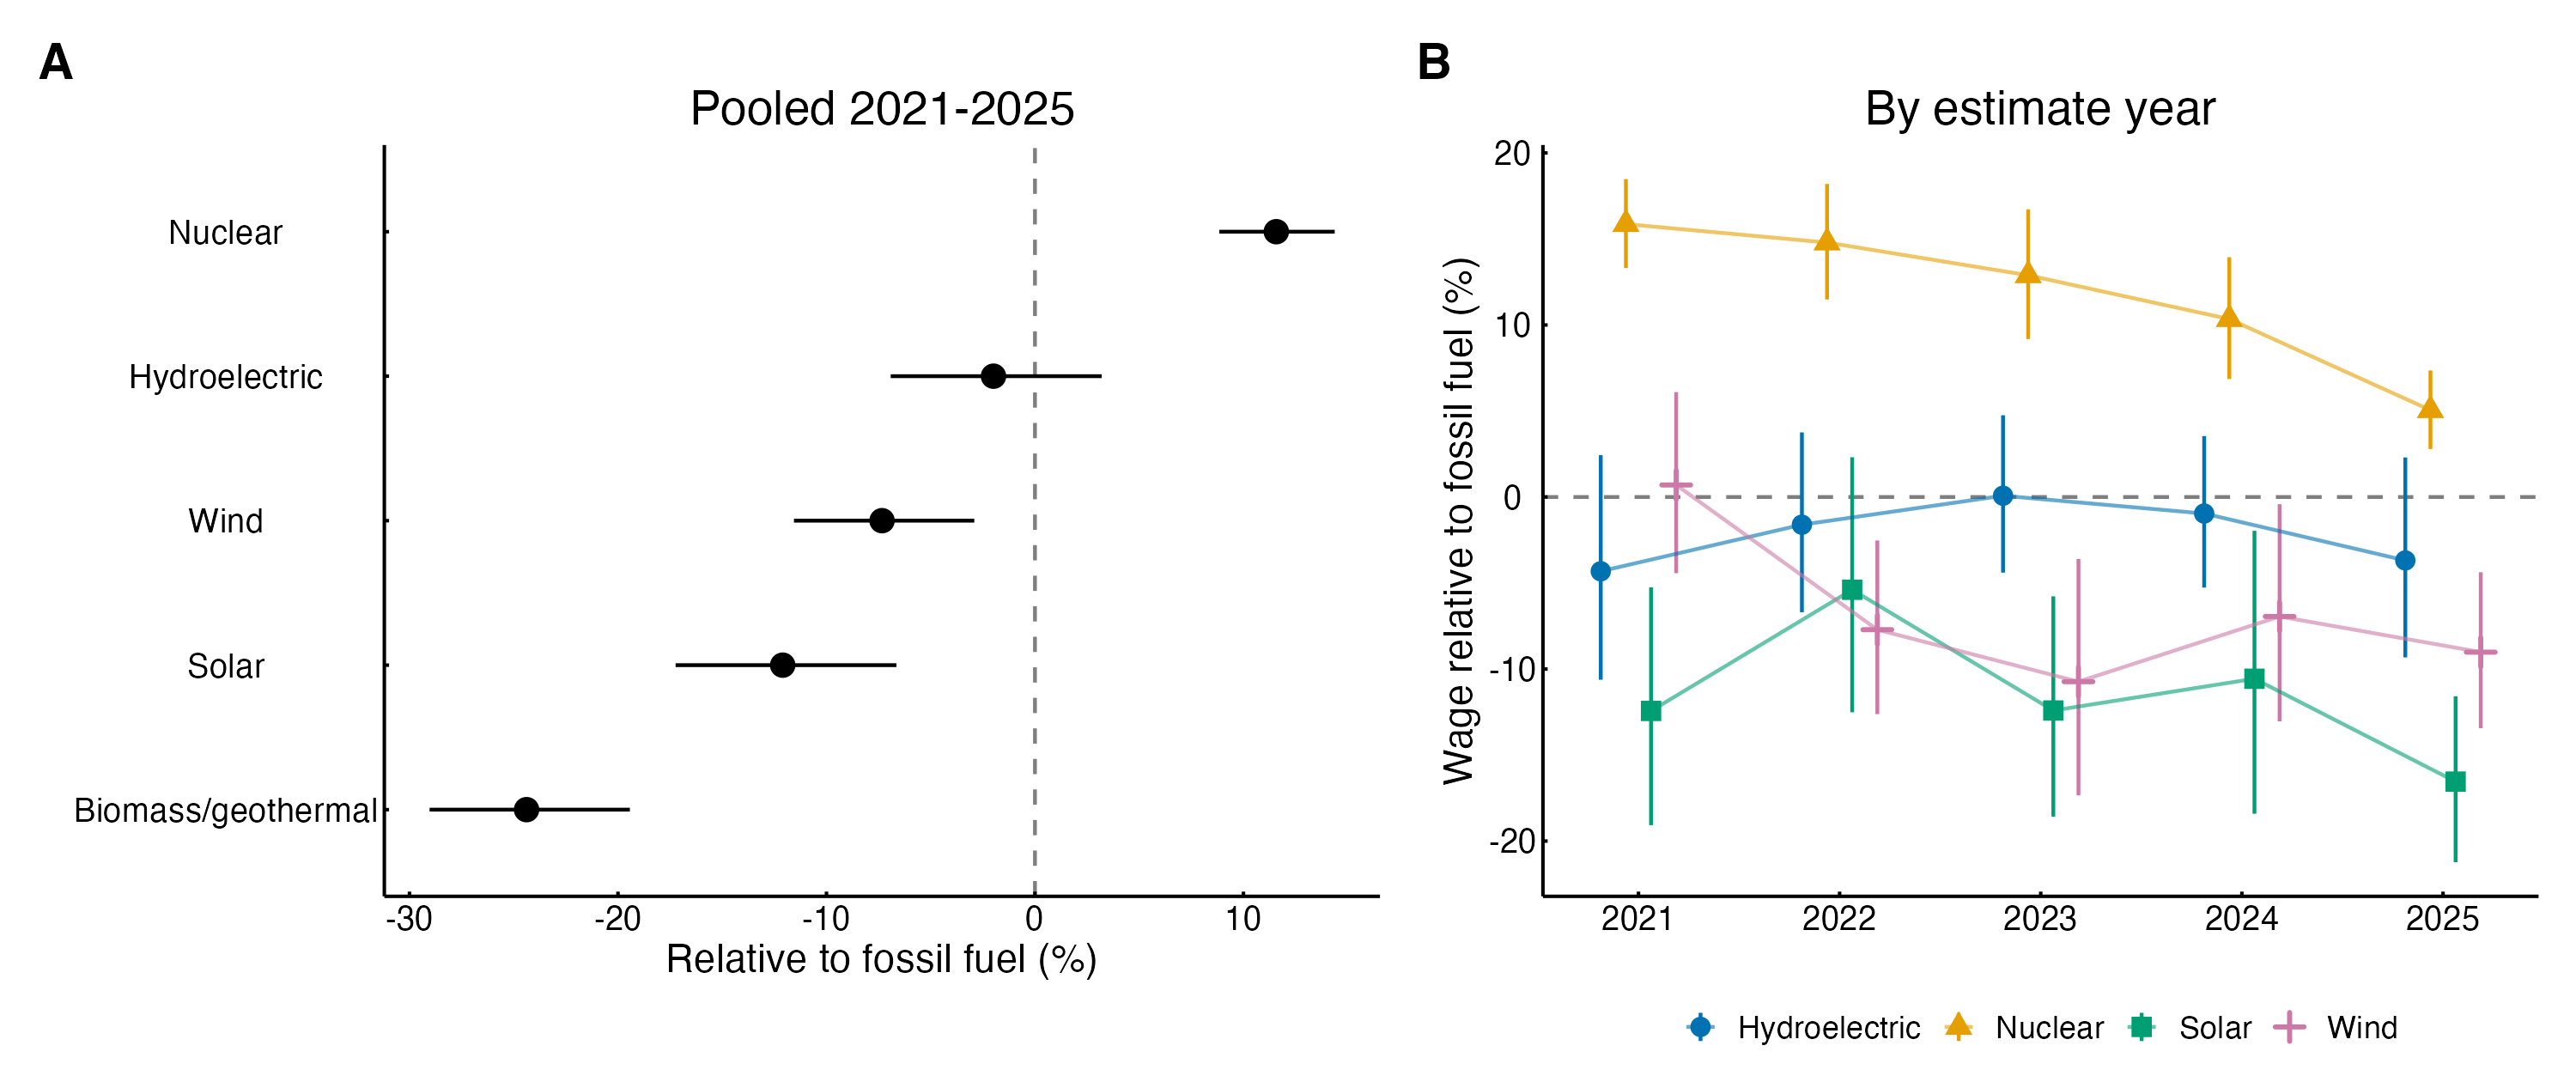
\includegraphics[width=0.95\linewidth,height=\textheight,keepaspectratio,alt={Fig. 1. Wage gaps by generation technology relative to fossil-fuel generation, same detailed occupation and survey round. (a) Pooled 2021--2025 estimates (model M4). (b) Estimates by survey round (model M7; biomass and geothermal omitted for sparsity). Points are percent differences; bars are 95\% confidence intervals clustered by occupation. Adjacent rounds share survey panels and are not independent.}]{../figures/fig2-technology.png}
\caption{Fig. 1. Wage gaps by generation technology relative to
fossil-fuel generation, same detailed occupation and survey round. (a)
Pooled 2021--2025 estimates (model M4). (b) Estimates by survey round
(model M7; biomass and geothermal omitted for sparsity). Points are
percent differences; bars are 95\% confidence intervals clustered by
occupation. Adjacent rounds share survey panels and are not
independent.}
\end{figure}

Fig. 1b traces the technology gaps across rounds. Two patterns stand
out, though adjacent rounds share most of their survey panels. First,
the nuclear premium over fossil-fuel generation narrowed steadily, from
15.9\% in May 2021 to 5.0\% in May 2025, as nuclear real pay fell (Table
1). Second, solar and wind did not converge on fossil-fuel pay. The
solar gap was −12.4\% in 2021 and −16.5\% in 2025, and wind moved from
parity in 2021 (+0.7\%) to −9.0\% in 2025.

\subsubsection{4.4 Occupations: penalties concentrated in blue-collar
trades}\label{occupations-penalties-concentrated-in-blue-collar-trades}

The renewable penalty differed across occupational classes (joint Wald
test of equal gaps, \emph{p} = 0.004; Fig. 2a). It was 16.4\% for
blue-collar trades (95\% CI −20.5\% to −12.0\%), 12.6\% for office and
administrative support, and 5.5\% for professional and managerial
occupations (−9.5\% to −1.4\%). The pre-specified contrast between
blue-collar and professional/managerial gaps was −0.122 log points (wild
bootstrap \emph{p} = 0.008), so blue-collar workers face a gap three
times as large, which supports H3. Separating managers from other
professional and technical occupations gives gaps of 3.5\% and 6.6\% for
these groups.

\begin{figure}
\centering
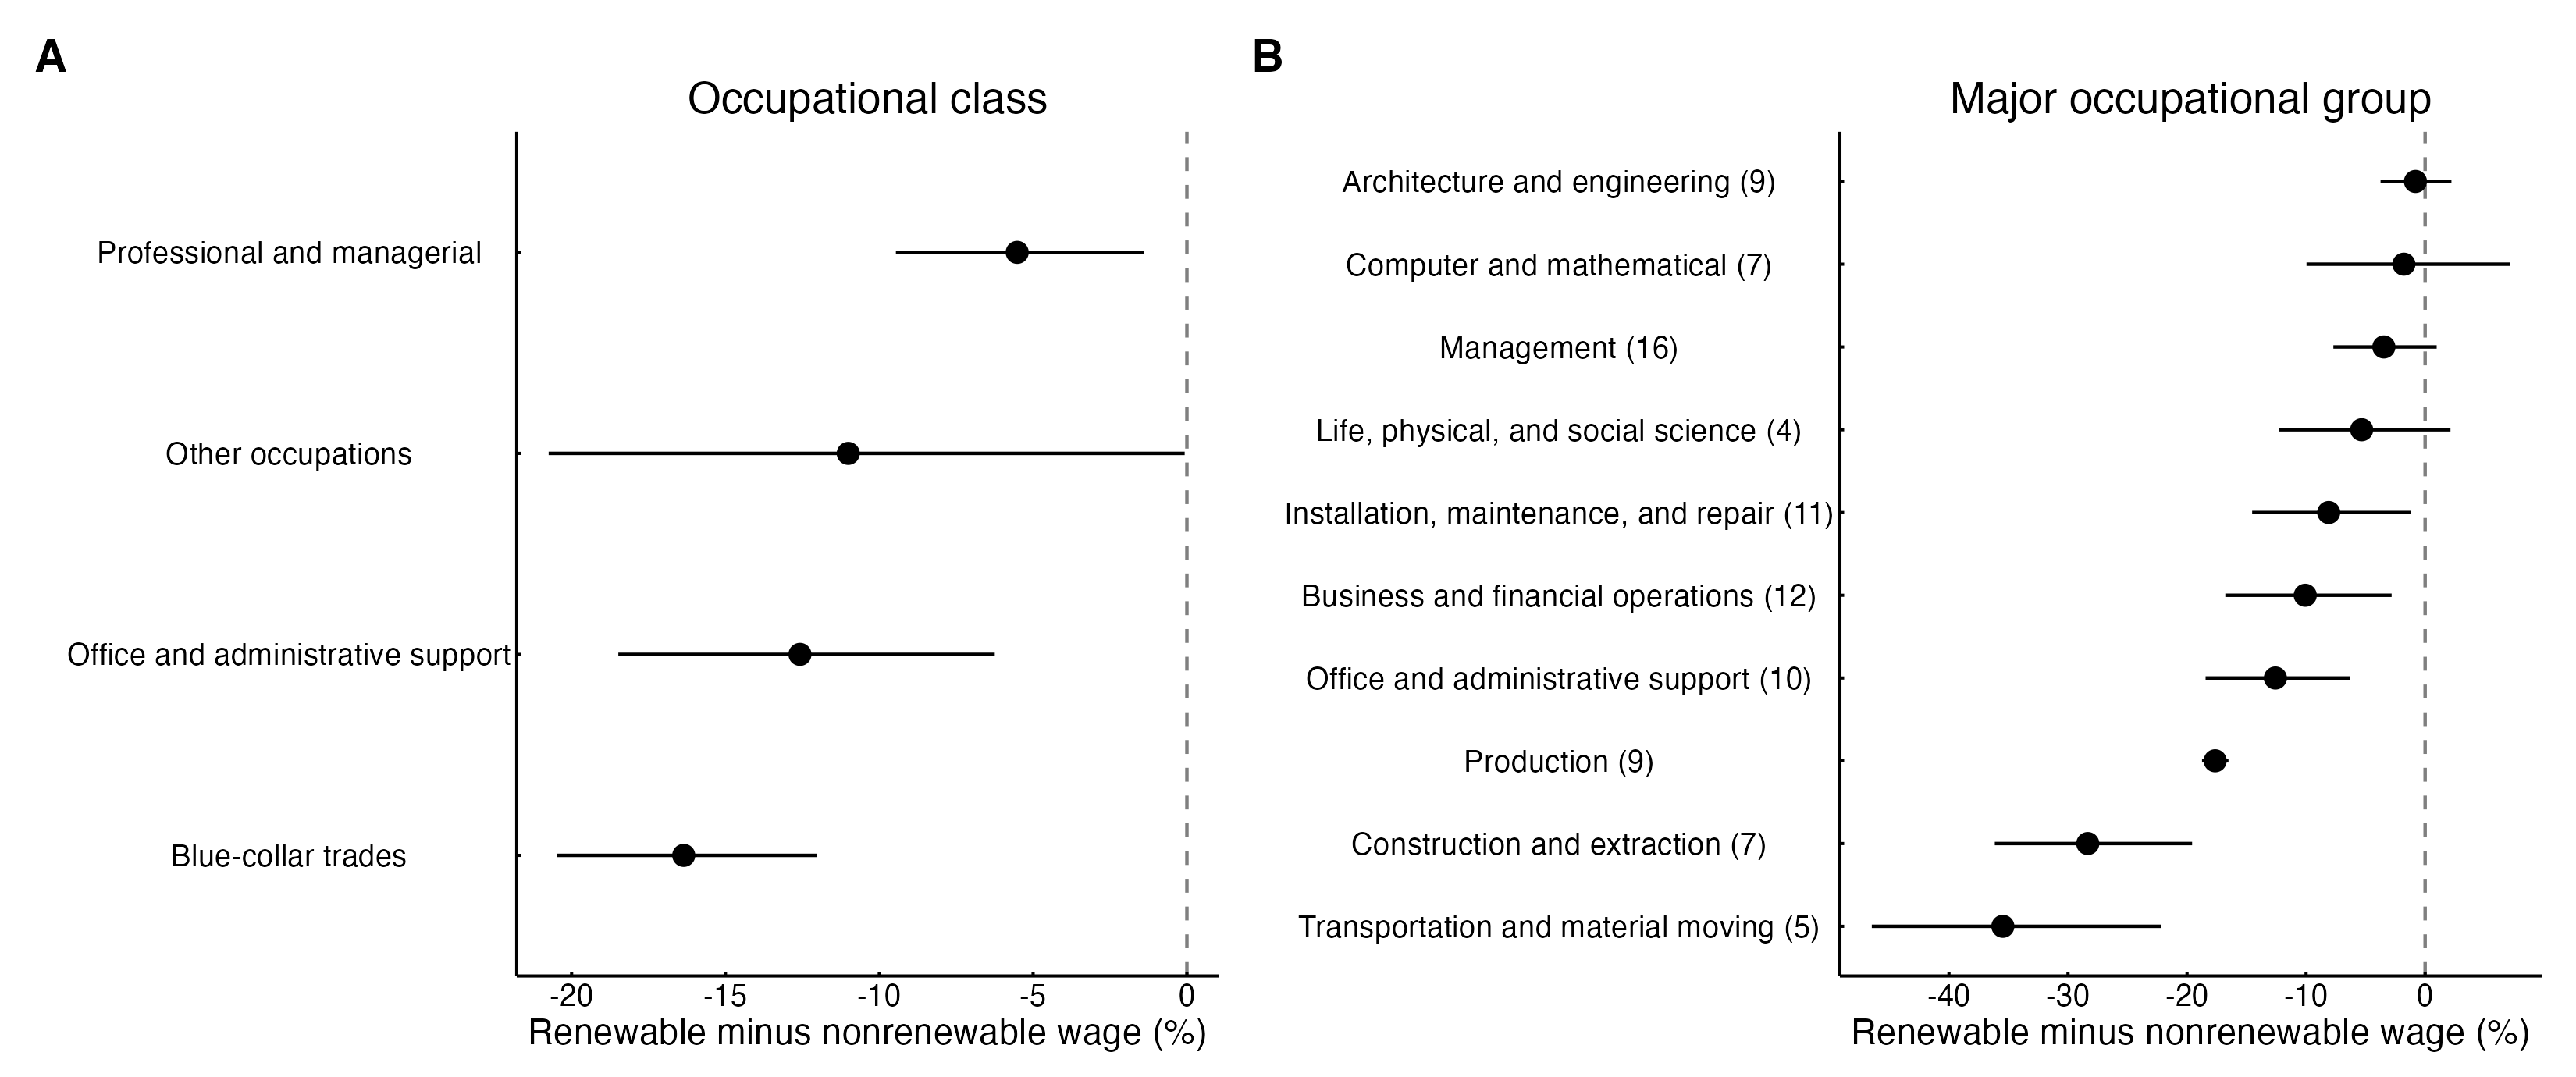
\includegraphics[width=0.9\linewidth,height=\textheight,keepaspectratio,alt={Fig. 2. Renewable minus nonrenewable wage gaps within detailed occupation and survey round, by (a) occupational class (model M5) and (b) SOC major group (major groups identified by at least three occupations observed in both sectors; number of such occupations in parentheses). Bars are 95\% confidence intervals clustered by occupation; intervals for groups with few occupations are approximate.}]{../figures/fig3-occupation.png}
\caption{Fig. 2. Renewable minus nonrenewable wage gaps within detailed
occupation and survey round, by (a) occupational class (model M5) and
(b) SOC major group (major groups identified by at least three
occupations observed in both sectors; number of such occupations in
parentheses). Bars are 95\% confidence intervals clustered by
occupation; intervals for groups with few occupations are approximate.}
\end{figure}

The major-group detail in Fig. 2b makes the gradient concrete. In
architecture and engineering occupations, renewable and nonrenewable
plants paid essentially the same (−0.8\%), and the management gap was
small (−3.5\%). Gaps were large in construction and extraction
(−28.3\%), transportation and material moving (−35.5\%), and production
(−17.6\%), where power-plant operators and related jobs are classified,
and moderate in installation, maintenance, and repair (−8.1\%).
Engineers at renewable plants are paid close to their fossil-fuel
counterparts; operators, technicians, and laborers are not.

Distributional checks point the same way: the gap was 19.8\% at the 10th
percentile of within-cell wages, 14.1\% at the median, and 5.9\% at the
90th percentile (Appendix Table A1). These are reported within-cell
percentiles, not worker-level quantiles, and top-coding compresses the
upper tail, but the pattern is consistent with stronger wage floors in
nonrenewable plants.

\subsubsection{4.5 Change over time: persistence, not
convergence}\label{change-over-time-persistence-not-convergence}

Fig. 3 plots the gaps by round. The regression-based within-occupation
gap (M6) was −0.121 log points in May 2021 and −0.139 in May 2025. The
pre-specified change between these rounds, which share no survey panels,
was −0.019 log points (95\% CI −0.055 to 0.018; wild bootstrap \emph{p}
= 0.330). Its 90\% interval (−0.049 to 0.012) lies within the ±0.05
equivalence margin, so by the pre-specified rule the gap was stable: any
narrowing larger than about five percent can be ruled out. The secondary
contrast between May 2021 and May 2024 gives the same conclusion
(+0.008; 90\% CI −0.029 to 0.044). Year-specific gaps were not identical
across all five rounds (joint Wald \emph{p} = 0.040), mainly because the
gap was smaller in May 2022 (−0.105) and larger in May 2025 (−0.139);
the May 2022 round shares four of its six panels with May 2021. H4 is
supported: rapid growth and new subsidies did not close the
within-occupation pay gap.

\begin{figure}
\centering
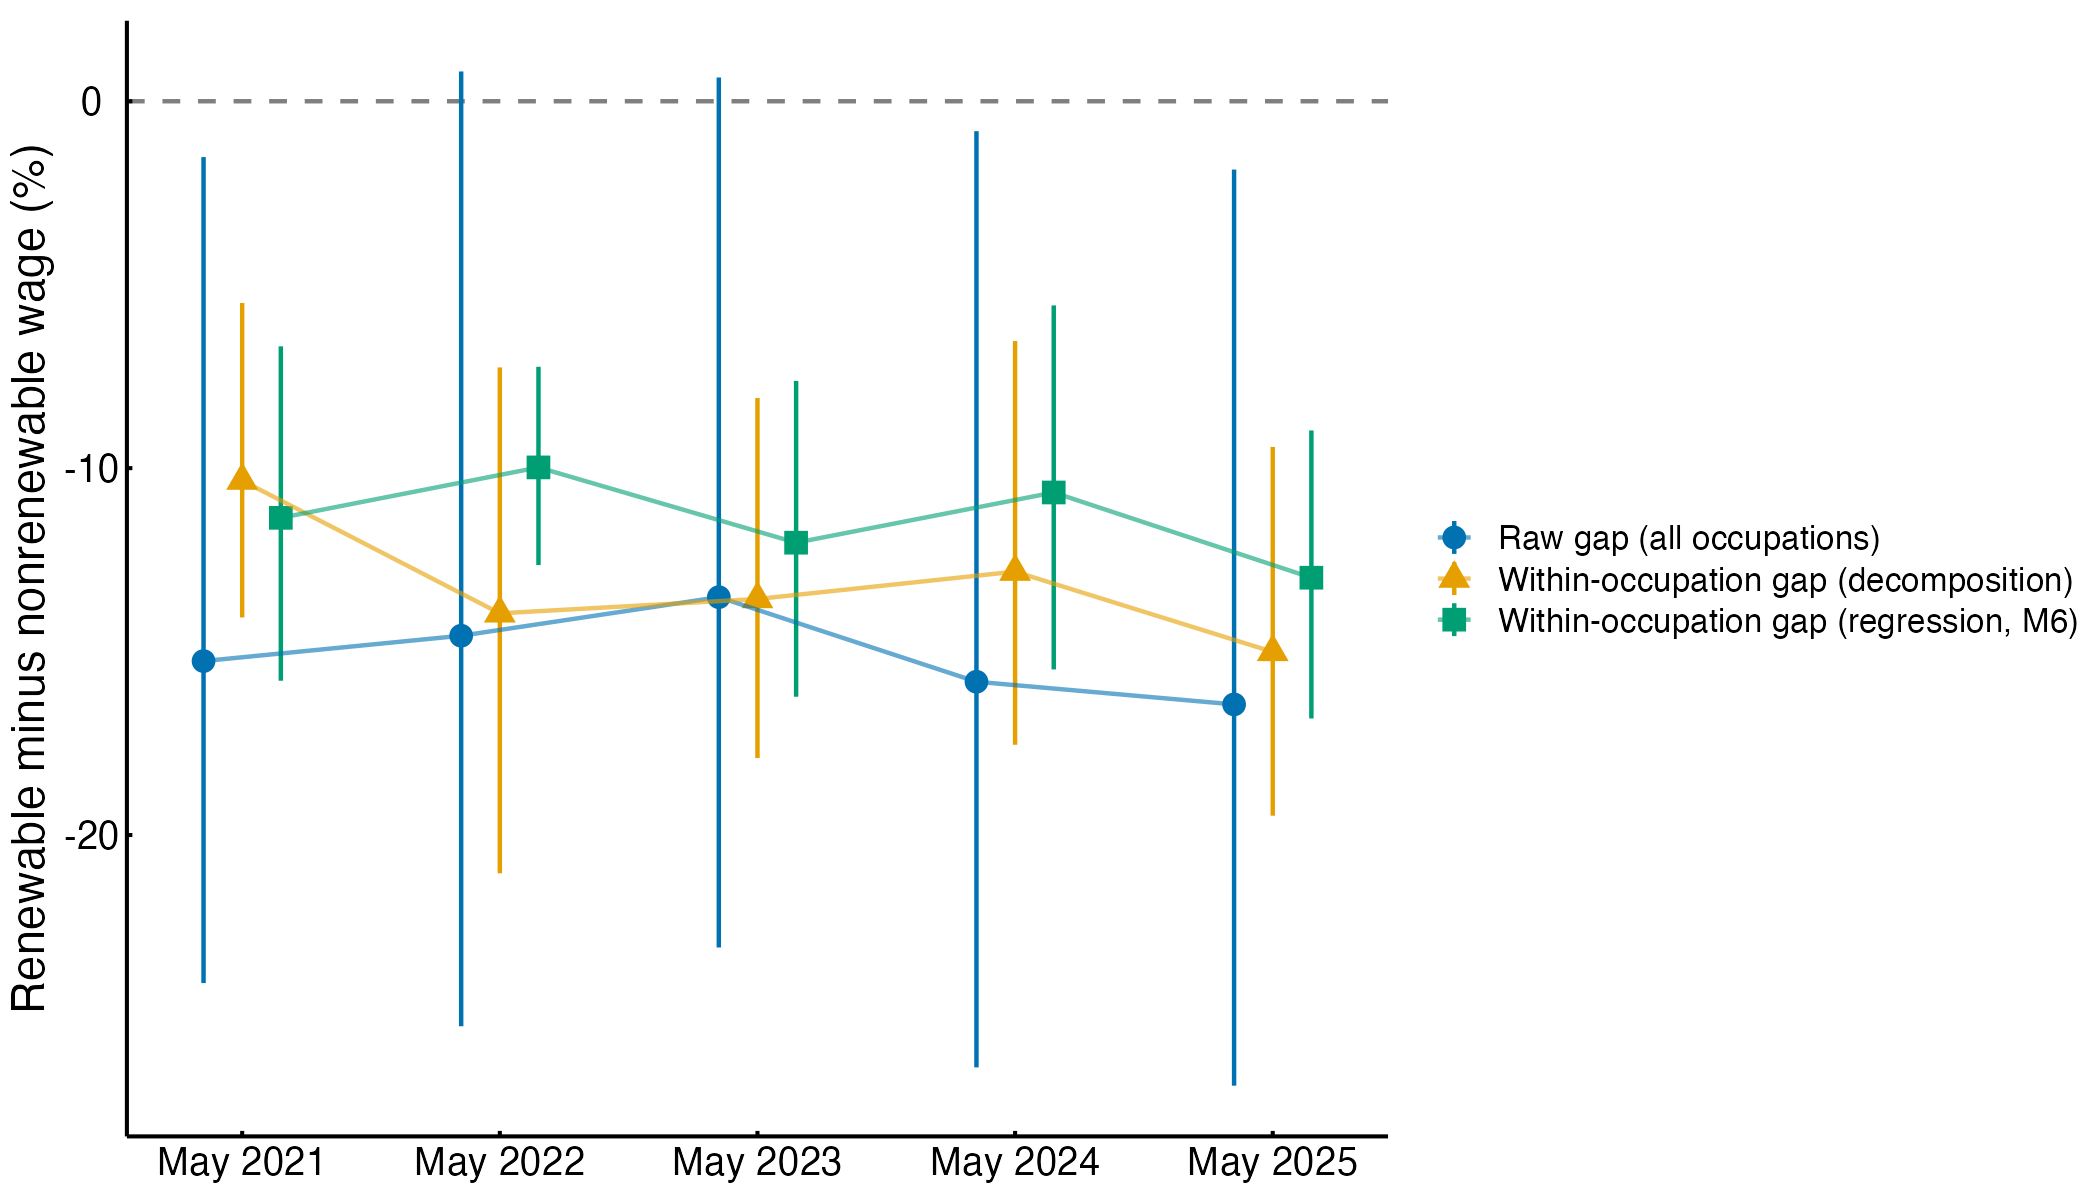
\includegraphics[width=0.9\linewidth,height=\textheight,keepaspectratio,alt={Fig. 3. Renewable minus nonrenewable wage gap by survey round: raw gap in employment-weighted mean log wages, within-occupation gap from the Kitagawa decomposition, and within-occupation gap from the regression model with occupation-by-round fixed effects (M6). Bars are 95\% bootstrap (decomposition) or cluster-robust (regression) confidence intervals. May 2021 and May 2025 estimates share no survey panels; adjacent rounds do.}]{../figures/fig1-gap-trend.png}
\caption{Fig. 3. Renewable minus nonrenewable wage gap by survey round:
raw gap in employment-weighted mean log wages, within-occupation gap
from the Kitagawa decomposition, and within-occupation gap from the
regression model with occupation-by-round fixed effects (M6). Bars are
95\% bootstrap (decomposition) or cluster-robust (regression) confidence
intervals. May 2021 and May 2025 estimates share no survey panels;
adjacent rounds do.}
\end{figure}

The worker-weighted decomposition suggests that, if anything, the gap
widened. The within-occupation term moved from −0.109 in 2021 to −0.163
in 2025, a change of −0.053 log points (bootstrap 95\% CI −0.112 to
−0.001). Splitting this change shows where it comes from. Pay changes
within the 54 occupations observed in both sectors in both rounds
contributed only −0.020, and shifting employment among them contributed
+0.018. The rest (−0.051) reflects the 23 occupations that entered
common support by 2025, net of 5 that left, as the growing solar and
wind workforces became large enough for BLS to publish more occupation
cells; on average these entering occupations carry larger renewable
penalties. The widening thus reflects renewable employment broadening
into occupations with large penalties more than deteriorating pay within
continuing occupations. Measured against fossil fuel alone (excluding
nuclear, whose premium shrank), the regression change was −0.040 (95\%
CI −0.080 to 0.000), again pointing toward persistence or modest
widening rather than convergence.

\subsubsection{4.6 Robustness}\label{robustness}

The within-occupation gap is negative and statistically significant in
all sixteen alternative specifications (Appendix Table A1), from −0.060
(90th percentile) to −0.220 (10th percentile) log points, including
−0.106 in cells present in all five rounds, −0.123 without weights, and
−0.118 after dropping the five largest identifying occupations. No
specification shows a significant narrowing between 2021 and 2025; the
estimated change ranges from −0.049 to +0.015 log points, and every 95\%
interval includes zero.

\subsection{5. Discussion}\label{discussion}

The question motivating this study was whether the jobs created by the
expansion of renewable electricity pay like the jobs they partly
replace. For the in-house workforces of U.S. generation plants in
2021--2025, the answer is no. Workers in the same detailed occupation
were paid about 11.5\% less in renewable establishments than in
fossil-fuel and nuclear establishments, the gap did not narrow while
renewable employment doubled, and it was largest for the operators,
technicians, mechanics, and laborers whose skills most closely match
those of workers leaving coal and gas plants. These findings fit
employer-based evidence that clean-energy firms pay no more than legacy
firms once education is held constant
{[}\citeproc{ref-colmer2025nice}{5}{]} and qualify occupation-based
findings that renewable jobs are well paid
{[}\citeproc{ref-curtis2023green}{4}{]}: renewable hiring does sit in
well-paid occupations, but renewable establishments pay those
occupations less, so measures that assign every worker the occupation's
average wage overstate what renewable employers pay.

The technology results speak to the theoretical argument. If the penalty
reflected something intrinsic to ``green'' work, such as lower
productivity, greater task simplicity, or the novelty of renewable
skills, hydroelectric generation should share it. It does not.
Hydroelectric pay is statistically indistinguishable from fossil-fuel
pay, while solar and wind, the newest and fastest-growing technologies,
pay significantly less than both fossil fuel and hydro. The dividing
line runs between legacy and new technologies, which is what an
organizational account of pay-setting predicts
{[}\citeproc{ref-tomaskovicdevey2019relational}{9},\citeproc{ref-winner1980artifacts}{37}{]}.
Published union and project-labor coverage rates are broadly consistent
with this ordering: about 19\% in nuclear generation, 16--17\% in coal
and natural gas, 13\% in water power, 12\% in wind, and 11--14\% in
solar generation {[}\citeproc{ref-doe2024useer}{11}{]}. The premium in
nuclear plants, the most institutionally consolidated technology, also
fits. The correspondence is loose: hydroelectric coverage resembles wind
coverage, yet only wind shows a gap, and the coverage figures refer to a
broader workforce. Union coverage alone cannot be the mechanism; plant
vintage, utility ownership, internal job ladders, and regional labor
markets are plausible complements. The institutional interpretation is
consistent with the patterns but untested.

The occupational gradient sharpens the just-transition stakes. Engineers
and managers carry their market value across technologies: renewable and
fossil-fuel plants pay them about the same. The penalty falls on manual
and craft workers, and it is larger at the bottom of within-cell wage
distributions than at the top. This is where collective bargaining and
internal labor markets have historically raised and compressed pay
{[}\citeproc{ref-kalleberg2011good}{19},\citeproc{ref-western2011unions}{33}{]},
and where union members fear that renewable jobs will not carry legacy
protections
{[}\citeproc{ref-sicotte2022necessary}{18},\citeproc{ref-sicotte2025labor}{39}{]}.
A fossil-fuel power-plant operator or construction-and-extraction worker
who moves to a solar or wind plant in the same occupation should expect
to earn substantially less, on average. Combined with evidence that few
workers make that move at all
{[}\citeproc{ref-curtis2024workers}{21}{]}, this suggests the
transition's labor-market costs are borne disproportionately by manual
workers, the group whose protection motivated the just-transition idea
{[}\citeproc{ref-ilo2014just}{12},\citeproc{ref-newell2013political}{13}{]}.

The persistence result bears on the ecological-modernization expectation
that growth and policy support would pull renewable pay up
{[}\citeproc{ref-spaargaren1992sociology}{10}{]}. Between survey rounds
that share no data, the within-occupation gap changed by less than two
percentage points, and a narrowing of more than about five percent can
be ruled out. The worker-weighted gap widened as the renewable workforce
broadened into occupations with large penalties. Two cautions apply.
First, the OEWS estimates for 2025 still include panels collected before
most 2022 policy changes could affect operations staffing, and wage
aging smooths change, so the window may be too short to see later
effects. Second, to the extent that the labor standards attached to the
new clean-electricity tax credits apply mainly to construction,
alteration, and repair work, they would not directly reach the permanent
operations workforce studied here. Even so, through May 2025 the
expansion reproduced the legacy pay hierarchy instead of eroding it
{[}\citeproc{ref-tilly1998durable}{8},\citeproc{ref-york2003key}{41}{]}.
The declining nuclear premium is a separate pattern that this study
cannot explain and that deserves direct study.

\subsubsection{5.1 Limitations}\label{limitations}

The estimates are descriptive: workers are compared within the same
classification, not the same tenure, region, or employer size. Wind and
solar plants are likely to be sited in more rural areas with lower
prevailing wages, and their workforces are newer, so part of the gap may
reflect geography and seniority rather than pay-setting for identical
work. State-by-industry tables or linked employer-employee data could
separate these explanations. The sample is limited to private, in-house
employees of generation establishments. It excludes publicly owned
utilities, including federal and municipal hydroelectric plants, and the
much larger construction and installation workforce, whose pay is shaped
by project labor agreements and prevailing-wage rules. Results may
differ for these groups. Suppression removes more renewable than
nonrenewable employment, although balanced-cell and
continuing-occupation analyses suggest it does not drive the headline
gap. Because OEWS rounds pool three years of panels, trend inferences
rest on two non-overlapping comparisons with limited power. Finally, the
hypotheses were developed after the author had seen a 2025 cross-section
and were not preregistered.

\subsection{6. Conclusion}\label{conclusion}

Renewable electricity generation in the United States grew rapidly in
the early 2020s, but the jobs it created inside generation plants paid
about 11.5\% less than fossil-fuel and nuclear jobs in the same
occupation, and this gap did not shrink as renewable employment doubled.
The penalty is not a property of renewable energy as such. It is
concentrated in the newer solar, wind, and biomass and geothermal
technologies, absent in long-established hydroelectric plants, and borne
mainly by blue-collar workers. For a just transition, job counts are not
enough. Policies that attach wage and bargaining standards to the
permanent operations workforce of new generation, not only to
construction, and that help displaced fossil-fuel workers carry their
pay and protections into renewable plants, would address the gap this
study documents. Future work should test the institutional mechanisms
directly, using plant ownership, union coverage, and worker tenure, and
should track whether the gap closes as renewable operations workforces
mature.

\subsection{Declarations}\label{declarations}

\textbf{Data availability.} All data are public: BLS Occupational
Employment and Wage Statistics national industry-specific estimates (May
2021--2025) and CPI-U series CUUR0000SA0. Analysis code (R) that
reproduces every table and figure from the raw BLS files is provided in
the replication materials.

\textbf{Declaration of generative AI use.} During the preparation of
this work the author used an AI assistant (Claude, Anthropic) to search
and verify literature, write and review analysis code, and draft and
edit text. The author reviewed and edited all content and takes full
responsibility for the publication.

\textbf{Competing interests.} The author declares no competing
interests.

\textbf{Funding.} This research received no specific funding.

\textbf{CRediT authorship contribution statement.} {[}Author{]}:
Conceptualization, Methodology, Formal analysis, Data curation, Writing
-- original draft, Writing -- review and editing.

\subsection{References}\label{references}

\protect\phantomsection\label{refs}
\begin{CSLReferences}{0}{0}
\bibitem[\citeproctext]{ref-stevis2015global}
\CSLLeftMargin{{[}1{]} }%
\CSLRightInline{D. Stevis, R. Felli, Global labour unions and just
transition to a green economy, International Environmental Agreements:
Politics, Law and Economics 15 (2015) 29--43.
https://doi.org/\href{https://doi.org/10.1007/s10784-014-9266-1}{10.1007/s10784-014-9266-1}.}

\bibitem[\citeproctext]{ref-mccauley2018just}
\CSLLeftMargin{{[}2{]} }%
\CSLRightInline{D. McCauley, R. Heffron, Just transition: Integrating
climate, energy and environmental justice, Energy Policy 119 (2018)
1--7.
https://doi.org/\href{https://doi.org/10.1016/j.enpol.2018.04.014}{10.1016/j.enpol.2018.04.014}.}

\bibitem[\citeproctext]{ref-vona2019measures}
\CSLLeftMargin{{[}3{]} }%
\CSLRightInline{F. Vona, G. Marin, D. Consoli, Measures, drivers and
effects of green employment: Evidence from US local labor markets,
2006--2014, Journal of Economic Geography 19 (2019) 1021--1048.
https://doi.org/\href{https://doi.org/10.1093/jeg/lby038}{10.1093/jeg/lby038}.}

\bibitem[\citeproctext]{ref-curtis2023green}
\CSLLeftMargin{{[}4{]} }%
\CSLRightInline{E.M. Curtis, I. Marinescu, Green energy jobs in the
united states: What are they, and where are they?, Environmental and
Energy Policy and the Economy 4 (2023) 202--237.
https://doi.org/\href{https://doi.org/10.1086/722677}{10.1086/722677}.}

\bibitem[\citeproctext]{ref-colmer2025nice}
\CSLLeftMargin{{[}5{]} }%
\CSLRightInline{J. Colmer, E. Lyubich, J.L. Voorheis, Nice work if you
can get it? The distribution of employment and earnings during the early
years of the clean energy transition, Centre for Economic Performance,
London School of Economics; Elsevier BV, 2025.
https://doi.org/\href{https://doi.org/10.2139/ssrn.5582530}{10.2139/ssrn.5582530}.}

\bibitem[\citeproctext]{ref-krueger1988efficiency}
\CSLLeftMargin{{[}6{]} }%
\CSLRightInline{A.B. Krueger, L.H. Summers, Efficiency wages and the
inter-industry wage structure, Econometrica 56 (1988) 259--293.
https://doi.org/\href{https://doi.org/10.2307/1911072}{10.2307/1911072}.}

\bibitem[\citeproctext]{ref-card2013workplace}
\CSLLeftMargin{{[}7{]} }%
\CSLRightInline{D. Card, J. Heining, P. Kline, Workplace heterogeneity
and the rise of west german wage inequality*, The Quarterly Journal of
Economics 128 (2013) 967--1015.
https://doi.org/\href{https://doi.org/10.1093/qje/qjt006}{10.1093/qje/qjt006}.}

\bibitem[\citeproctext]{ref-tilly1998durable}
\CSLLeftMargin{{[}8{]} }%
\CSLRightInline{C. Tilly, Durable inequality, University of California
Press, Berkeley, 1998.}

\bibitem[\citeproctext]{ref-tomaskovicdevey2019relational}
\CSLLeftMargin{{[}9{]} }%
\CSLRightInline{D. Tomaskovic-Devey, D. Avent-Holt, Relational
inequalities: An organizational approach, Oxford University Press, New
York, 2019.}

\bibitem[\citeproctext]{ref-spaargaren1992sociology}
\CSLLeftMargin{{[}10{]} }%
\CSLRightInline{G. Spaargaren, A.P.J. Mol, Sociology, environment, and
modernity: Ecological modernization as a theory of social change,
Society \& Natural Resources 5 (1992) 323--344.
https://doi.org/\href{https://doi.org/10.1080/08941929209380797}{10.1080/08941929209380797}.}

\bibitem[\citeproctext]{ref-doe2024useer}
\CSLLeftMargin{{[}11{]} }%
\CSLRightInline{U.S. Department of Energy, United states energy and
employment report 2024, U.S. Department of Energy, Washington, DC, 2024.
\url{https://www.energy.gov/sites/default/files/2024-10/USEER\%202024_COMPLETE_1002.pdf}.}

\bibitem[\citeproctext]{ref-ilo2014just}
\CSLLeftMargin{{[}12{]} }%
\CSLRightInline{International Labour Office, Editorial: A just
transition for all: Can the past inform the future?, International
Journal of Labour Research 6 (2014) 173--185.}

\bibitem[\citeproctext]{ref-newell2013political}
\CSLLeftMargin{{[}13{]} }%
\CSLRightInline{P. Newell, D. Mulvaney, The political economy of the
{``just transition,''} The Geographical Journal 179 (2013) 132--140.
https://doi.org/\href{https://doi.org/10.1111/geoj.12008}{10.1111/geoj.12008}.}

\bibitem[\citeproctext]{ref-healy2017politicizing}
\CSLLeftMargin{{[}14{]} }%
\CSLRightInline{N. Healy, J. Barry, Politicizing energy justice and
energy system transitions: Fossil fuel divestment and a {``just
transition,''} Energy Policy 108 (2017) 451--459.
https://doi.org/\href{https://doi.org/10.1016/j.enpol.2017.06.014}{10.1016/j.enpol.2017.06.014}.}

\bibitem[\citeproctext]{ref-beckfield2023social}
\CSLLeftMargin{{[}15{]} }%
\CSLRightInline{J. Beckfield, D.A. Evrard, The social impacts of
supply-side decarbonization, Annual Review of Sociology 49 (2023)
155--175.
https://doi.org/\href{https://doi.org/10.1146/annurev-soc-031021-012201}{10.1146/annurev-soc-031021-012201}.}

\bibitem[\citeproctext]{ref-carley2020justice}
\CSLLeftMargin{{[}16{]} }%
\CSLRightInline{S. Carley, D.M. Konisky, The justice and equity
implications of the clean energy transition, Nature Energy 5 (2020)
569--577.
https://doi.org/\href{https://doi.org/10.1038/s41560-020-0641-6}{10.1038/s41560-020-0641-6}.}

\bibitem[\citeproctext]{ref-raimi2022mapping}
\CSLLeftMargin{{[}17{]} }%
\CSLRightInline{D. Raimi, S. Carley, D. Konisky, Mapping county-level
vulnerability to the energy transition in US fossil fuel communities,
Scientific Reports 12 (2022).
https://doi.org/\href{https://doi.org/10.1038/s41598-022-19927-6}{10.1038/s41598-022-19927-6}.}

\bibitem[\citeproctext]{ref-sicotte2022necessary}
\CSLLeftMargin{{[}18{]} }%
\CSLRightInline{D.M. Sicotte, K.A. Joyce, A. Hesse, Necessary, welcome
or dreaded? Insights on low-carbon transitions from unionized energy
workers in the united states, Energy Research \& Social Science 88
(2022) 102511.
https://doi.org/\href{https://doi.org/10.1016/j.erss.2022.102511}{10.1016/j.erss.2022.102511}.}

\bibitem[\citeproctext]{ref-kalleberg2011good}
\CSLLeftMargin{{[}19{]} }%
\CSLRightInline{A.L. Kalleberg, Good jobs, bad jobs: The rise of
polarized and precarious employment systems in the united states,
1970s--2000s, Russell Sage Foundation, New York, 2011.}

\bibitem[\citeproctext]{ref-kuai2025estimating}
\CSLLeftMargin{{[}20{]} }%
\CSLRightInline{W. Kuai, R.J.R. Elliott, T. Okubo, C. Ozgen, Estimating
the green wage premium, IZA Institute of Labor Economics; Elsevier BV,
2025.
https://doi.org/\href{https://doi.org/10.2139/ssrn.5240989}{10.2139/ssrn.5240989}.}

\bibitem[\citeproctext]{ref-curtis2024workers}
\CSLLeftMargin{{[}21{]} }%
\CSLRightInline{E.M. Curtis, L. O'Kane, R.J. Park, Workers and the
green-energy transition: Evidence from 300 million job transitions,
Environmental and Energy Policy and the Economy 5 (2024) 127--161.
https://doi.org/\href{https://doi.org/10.1086/727880}{10.1086/727880}.}

\bibitem[\citeproctext]{ref-godoy2025green}
\CSLLeftMargin{{[}22{]} }%
\CSLRightInline{A. Godøy, E.T. Isaksen, A green wage premium?, Grantham
Research Institute on Climate Change; the Environment, 2025.}

\bibitem[\citeproctext]{ref-lehmann2020wages}
\CSLLeftMargin{{[}23{]} }%
\CSLRightInline{S. Lehmann, Wages, benefits, and change: A supplemental
report to the annual u.s. Energy and employment report, BW Research
Partnership, National Association of State Energy Officials,; Energy
Futures Initiative, 2020.}

\bibitem[\citeproctext]{ref-bradley2025empirical}
\CSLLeftMargin{{[}24{]} }%
\CSLRightInline{P. Bradley, D. Whittard, E. Green, I. Brooks, R. Hanna,
Empirical research on green jobs: A review and reflection with
practitioners, Sustainable Futures 9 (2025) 100527.
https://doi.org/\href{https://doi.org/10.1016/j.sftr.2025.100527}{10.1016/j.sftr.2025.100527}.}

\bibitem[\citeproctext]{ref-hanna2024job}
\CSLLeftMargin{{[}25{]} }%
\CSLRightInline{R. Hanna, P. Heptonstall, R. Gross, Job creation in a
low carbon transition to renewables and energy efficiency: A review of
international evidence, Sustainability Science 19 (2024) 125--150.
https://doi.org/\href{https://doi.org/10.1007/s11625-023-01440-y}{10.1007/s11625-023-01440-y}.}

\bibitem[\citeproctext]{ref-pearse2022labour}
\CSLLeftMargin{{[}26{]} }%
\CSLRightInline{R. Pearse, G. Bryant, Labour in transition: A
value-theoretical approach to renewable energy labour, Environment and
Planning E: Nature and Space 5 (2022) 1872--1894.
https://doi.org/\href{https://doi.org/10.1177/25148486211055542}{10.1177/25148486211055542}.}

\bibitem[\citeproctext]{ref-abowd1999high}
\CSLLeftMargin{{[}27{]} }%
\CSLRightInline{J.M. Abowd, F. Kramarz, D.N. Margolis, High wage workers
and high wage firms, Econometrica 67 (1999) 251--333.
https://doi.org/\href{https://doi.org/10.1111/1468-0262.00020}{10.1111/1468-0262.00020}.}

\bibitem[\citeproctext]{ref-barth2016where}
\CSLLeftMargin{{[}28{]} }%
\CSLRightInline{E. Barth, A. Bryson, J.C. Davis, R. Freeman, It's where
you work: Increases in the dispersion of earnings across establishments
and individuals in the united states, Journal of Labor Economics 34
(2016) S67--S97.
https://doi.org/\href{https://doi.org/10.1086/684045}{10.1086/684045}.}

\bibitem[\citeproctext]{ref-song2019firming}
\CSLLeftMargin{{[}29{]} }%
\CSLRightInline{J. Song, D.J. Price, F. Guvenen, N. Bloom, T. von
Wachter, Firming up inequality*, The Quarterly Journal of Economics 134
(2019) 1--50.
https://doi.org/\href{https://doi.org/10.1093/qje/qjy025}{10.1093/qje/qjy025}.}

\bibitem[\citeproctext]{ref-tomaskovicdevey2020rising}
\CSLLeftMargin{{[}30{]} }%
\CSLRightInline{D. Tomaskovic-Devey, A. Rainey, D. Avent-Holt, N.
Bandelj, I. Boza, D. Cort, O. Godechot, G. Hajdu, M. Hällsten, L.F.
Henriksen, A.S. Hermansen, F. Hou, J. Jung, A. Kanjuo-Mrčela, J. King,
N. Kodama, T. Kristal, A. Křížková, Z. Lippényi, S.M. Melzer, E. Mun, A.
Penner, T. Petersen, A. Poje, M. Safi, M. Thaning, Z. Tufail, Rising
between-workplace inequalities in high-income countries, Proceedings of
the National Academy of Sciences 117 (2020) 9277--9283.
https://doi.org/\href{https://doi.org/10.1073/pnas.1918249117}{10.1073/pnas.1918249117}.}

\bibitem[\citeproctext]{ref-wilmers2021consolidated}
\CSLLeftMargin{{[}31{]} }%
\CSLRightInline{N. Wilmers, C. Aeppli, Consolidated advantage: New
organizational dynamics of wage inequality, American Sociological Review
86 (2021) 1100--1130.
https://doi.org/\href{https://doi.org/10.1177/00031224211049205}{10.1177/00031224211049205}.}

\bibitem[\citeproctext]{ref-weeden2002why}
\CSLLeftMargin{{[}32{]} }%
\CSLRightInline{K.A. Weeden, Why do some occupations pay more than
others? Social closure and earnings inequality in the united states,
American Journal of Sociology 108 (2002) 55--101.
https://doi.org/\href{https://doi.org/10.1086/344121}{10.1086/344121}.}

\bibitem[\citeproctext]{ref-western2011unions}
\CSLLeftMargin{{[}33{]} }%
\CSLRightInline{B. Western, J. Rosenfeld, Unions, norms, and the rise in
u.s. Wage inequality, American Sociological Review 76 (2011) 513--537.
https://doi.org/\href{https://doi.org/10.1177/0003122411414817}{10.1177/0003122411414817}.}

\bibitem[\citeproctext]{ref-rosenfeld2014unions}
\CSLLeftMargin{{[}34{]} }%
\CSLRightInline{J. Rosenfeld, What unions no longer do, Harvard
University Press, Cambridge, MA, 2014.}

\bibitem[\citeproctext]{ref-petersen1995separate}
\CSLLeftMargin{{[}35{]} }%
\CSLRightInline{T. Petersen, L.A. Morgan, Separate and unequal:
Occupation-establishment sex segregation and the gender wage gap,
American Journal of Sociology 101 (1995) 329--365.
https://doi.org/\href{https://doi.org/10.1086/230727}{10.1086/230727}.}

\bibitem[\citeproctext]{ref-cohen2003individuals}
\CSLLeftMargin{{[}36{]} }%
\CSLRightInline{P.N. Cohen, M.L. Huffman, Individuals, jobs, and labor
markets: The devaluation of women's work, American Sociological Review
68 (2003) 443--463.
https://doi.org/\href{https://doi.org/10.2307/1519732}{10.2307/1519732}.}

\bibitem[\citeproctext]{ref-winner1980artifacts}
\CSLLeftMargin{{[}37{]} }%
\CSLRightInline{L. Winner, Do artifacts have politics?, Daedalus 109
(1980) 121--136.}

\bibitem[\citeproctext]{ref-diprete2010compensation}
\CSLLeftMargin{{[}38{]} }%
\CSLRightInline{T.A. DiPrete, G.M. Eirich, M. Pittinsky, Compensation
benchmarking, leapfrogs, and the surge in executive pay, American
Journal of Sociology 115 (2010) 1671--1712.
https://doi.org/\href{https://doi.org/10.1086/652297}{10.1086/652297}.}

\bibitem[\citeproctext]{ref-sicotte2025labor}
\CSLLeftMargin{{[}39{]} }%
\CSLRightInline{D.M. Sicotte, U.s. Labor and renewable energy: Green
growth versus the green new deal, Environmental Sociology 11 (2025)
228--238.
https://doi.org/\href{https://doi.org/10.1080/23251042.2024.2422033}{10.1080/23251042.2024.2422033}.}

\bibitem[\citeproctext]{ref-vachon2023clean}
\CSLLeftMargin{{[}40{]} }%
\CSLRightInline{T.E. Vachon, Clean air and good jobs: U.s. Labor and the
struggle for climate justice, Temple University Press, Philadelphia,
2023.}

\bibitem[\citeproctext]{ref-york2003key}
\CSLLeftMargin{{[}41{]} }%
\CSLRightInline{R. York, E.A. Rosa, Key challenges to ecological
modernization theory: Institutional efficacy, case study evidence, units
of analysis, and the pace of eco-efficiency, Organization \& Environment
16 (2003) 273--288.
https://doi.org/\href{https://doi.org/10.1177/1086026603256299}{10.1177/1086026603256299}.}

\bibitem[\citeproctext]{ref-burke2018political}
\CSLLeftMargin{{[}42{]} }%
\CSLRightInline{M.J. Burke, J.C. Stephens, Political power and renewable
energy futures: A critical review, Energy Research \& Social Science 35
(2018) 78--93.
https://doi.org/\href{https://doi.org/10.1016/j.erss.2017.10.018}{10.1016/j.erss.2017.10.018}.}

\bibitem[\citeproctext]{ref-knuth2019whatever}
\CSLLeftMargin{{[}43{]} }%
\CSLRightInline{S. Knuth, Whatever happened to green collar jobs?
Populism and clean energy transition, Annals of the American Association
of Geographers 109 (2019) 634--643.
https://doi.org/\href{https://doi.org/10.1080/24694452.2018.1523001}{10.1080/24694452.2018.1523001}.}

\bibitem[\citeproctext]{ref-hess2012good}
\CSLLeftMargin{{[}44{]} }%
\CSLRightInline{D.J. Hess, Good green jobs in a global economy: Making
and keeping new industries in the united states, MIT Press, Cambridge,
MA, 2012.}

\bibitem[\citeproctext]{ref-cameron2008bootstrap}
\CSLLeftMargin{{[}45{]} }%
\CSLRightInline{A.C. Cameron, J.B. Gelbach, D.L. Miller, Bootstrap-based
improvements for inference with clustered errors, Review of Economics
and Statistics 90 (2008) 414--427.
https://doi.org/\href{https://doi.org/10.1162/rest.90.3.414}{10.1162/rest.90.3.414}.}

\bibitem[\citeproctext]{ref-mackinnon2017wild}
\CSLLeftMargin{{[}46{]} }%
\CSLRightInline{J.G. MacKinnon, M.D. Webb, Wild bootstrap inference for
wildly different cluster sizes, Journal of Applied Econometrics 32
(2016) 233--254.
https://doi.org/\href{https://doi.org/10.1002/jae.2508}{10.1002/jae.2508}.}

\bibitem[\citeproctext]{ref-webb2023reworking}
\CSLLeftMargin{{[}47{]} }%
\CSLRightInline{M.D. Webb, Reworking wild bootstrap‐based inference for
clustered errors, Canadian Journal of Economics/Revue Canadienne
d'économique 56 (2023) 839--858.
https://doi.org/\href{https://doi.org/10.1111/caje.12661}{10.1111/caje.12661}.}

\bibitem[\citeproctext]{ref-lakens2017equivalence}
\CSLLeftMargin{{[}48{]} }%
\CSLRightInline{D. Lakens, Equivalence tests: A practical primer for
\textless i\textgreater t\textless/i\textgreater{} tests, correlations,
and meta-analyses, Social Psychological and Personality Science 8 (2017)
355--362.
https://doi.org/\href{https://doi.org/10.1177/1948550617697177}{10.1177/1948550617697177}.}

\bibitem[\citeproctext]{ref-bls2025oews}
\CSLLeftMargin{{[}49{]} }%
\CSLRightInline{U.S. Bureau of Labor Statistics, Occupational employment
and wage statistics: Technical notes for may 2024 OEWS estimates,
(2025). \url{https://www.bls.gov/oes/current/oes_tec.htm}.}

\bibitem[\citeproctext]{ref-bls2025oewsfaq}
\CSLLeftMargin{{[}50{]} }%
\CSLRightInline{U.S. Bureau of Labor Statistics, Occupational employment
and wage statistics: Frequently asked questions, (2025).
\url{https://www.bls.gov/oes/oes_ques.htm}.}

\bibitem[\citeproctext]{ref-kitagawa1955components}
\CSLLeftMargin{{[}51{]} }%
\CSLRightInline{E.M. Kitagawa, Components of a difference between two
rates*, Journal of the American Statistical Association 50 (1955)
1168--1194.
https://doi.org/\href{https://doi.org/10.1080/01621459.1955.10501299}{10.1080/01621459.1955.10501299}.}

\end{CSLReferences}

\newpage

\subsection{Appendix}\label{appendix}

\textbf{Table A1.} Robustness of the within-occupation renewable wage
gap (model M3) and of the May 2025 minus May 2021 change (model M6).

{\def\LTcaptype{none} % do not increment counter
\begin{longtable}[]{@{}
  >{\raggedright\arraybackslash}p{(\linewidth - 6\tabcolsep) * \real{0.5528}}
  >{\raggedright\arraybackslash}p{(\linewidth - 6\tabcolsep) * \real{0.0407}}
  >{\raggedright\arraybackslash}p{(\linewidth - 6\tabcolsep) * \real{0.2033}}
  >{\raggedright\arraybackslash}p{(\linewidth - 6\tabcolsep) * \real{0.2033}}@{}}
\toprule\noalign{}
\begin{minipage}[b]{\linewidth}\raggedright
Specification
\end{minipage} & \begin{minipage}[b]{\linewidth}\raggedright
Cells
\end{minipage} & \begin{minipage}[b]{\linewidth}\raggedright
Gap (log points) {[}95\% CI{]}
\end{minipage} & \begin{minipage}[b]{\linewidth}\raggedright
Change 2025--2021 {[}95\% CI{]}
\end{minipage} \\
\midrule\noalign{}
\endhead
\bottomrule\noalign{}
\endlastfoot
Headline specification (M3 / M6) & 1578 & -0.122 {[}-0.164, -0.080{]} &
-0.019 {[}-0.055, 0.018{]} \\
R1 Balanced industry-occupation cells & 975 & -0.106 {[}-0.168,
-0.044{]} & 0.015 {[}-0.011, 0.041{]} \\
R2 Precision weights (employment / PRSE squared) & 1578 & -0.132
{[}-0.192, -0.071{]} & -0.012 {[}-0.105, 0.082{]} \\
R3 Unweighted & 1578 & -0.123 {[}-0.154, -0.092{]} & -0.009 {[}-0.062,
0.044{]} \\
R4 Median wage & 1578 & -0.152 {[}-0.200, -0.105{]} & 0.009 {[}-0.041,
0.059{]} \\
R5 10th-percentile wage & 1578 & -0.220 {[}-0.296, -0.145{]} & -0.004
{[}-0.077, 0.069{]} \\
R5 90th-percentile wage (top-coded) & 1578 & -0.060 {[}-0.086, -0.035{]}
& -0.049 {[}-0.104, 0.006{]} \\
R6 Other generation as renewable & 1709 & -0.115 {[}-0.162, -0.068{]} &
-0.038 {[}-0.083, 0.008{]} \\
R7 Other generation as nonrenewable & 1709 & -0.119 {[}-0.159, -0.079{]}
& -0.017 {[}-0.053, 0.020{]} \\
R8 Drop top-coded cells & 1577 & -0.122 {[}-0.164, -0.080{]} & -0.018
{[}-0.055, 0.018{]} \\
R9 Mean-wage PRSE at most 10 & 1456 & -0.128 {[}-0.173, -0.082{]} &
-0.014 {[}-0.048, 0.020{]} \\
R10 Nominal wages & 1578 & -0.122 {[}-0.164, -0.080{]} & -0.019
{[}-0.055, 0.018{]} \\
R11 2021 and 2025 only & 630 & -0.132 {[}-0.176, -0.088{]} & -0.019
{[}-0.055, 0.018{]} \\
R12 New renewables vs legacy (hydro grouped with fossil and nuclear) &
1578 & -0.164 {[}-0.218, -0.110{]} & -0.016 {[}-0.060, 0.029{]} \\
R13 Exclude nuclear & 1031 & -0.101 {[}-0.148, -0.053{]} & -0.040
{[}-0.080, 0.000{]} \\
R14 Hourly mean wage & 1578 & -0.122 {[}-0.164, -0.080{]} & -0.019
{[}-0.055, 0.018{]} \\
R15 Drop five largest identifying occupations & 1450 & -0.118 {[}-0.155,
-0.082{]} & -0.039 {[}-0.092, 0.014{]} \\
R16 SE clustered by industry-occupation cell & 1578 & -0.122 {[}-0.165,
-0.079{]} & -0.019 {[}-0.059, 0.022{]} \\
\end{longtable}
}

\emph{Note:} Log points; 95\% confidence intervals clustered by detailed
occupation (R16: by industry-by-occupation cell). Percentile outcomes
are reported within-cell percentiles; the 90th percentile is top-coded
in some legacy cells. R10 and R14 coincide with the headline estimate
because occupation-by-round fixed effects absorb the CPI deflator and
the 2,080-hour annualization. R11 reproduces the headline change because
round-specific fixed effects make each round's gap estimable from that
round alone.

\textbf{Table A2.} Main regression models (coefficients in log points;
standard errors clustered by detailed occupation in parentheses).

{\def\LTcaptype{none} % do not increment counter
\begin{longtable}[]{@{}
  >{\raggedright\arraybackslash}p{(\linewidth - 12\tabcolsep) * \real{0.1429}}
  >{\raggedright\arraybackslash}p{(\linewidth - 12\tabcolsep) * \real{0.1429}}
  >{\raggedright\arraybackslash}p{(\linewidth - 12\tabcolsep) * \real{0.1429}}
  >{\raggedright\arraybackslash}p{(\linewidth - 12\tabcolsep) * \real{0.1429}}
  >{\raggedright\arraybackslash}p{(\linewidth - 12\tabcolsep) * \real{0.1429}}
  >{\raggedright\arraybackslash}p{(\linewidth - 12\tabcolsep) * \real{0.1429}}
  >{\raggedright\arraybackslash}p{(\linewidth - 12\tabcolsep) * \real{0.1429}}@{}}
\toprule\noalign{}
\begin{minipage}[b]{\linewidth}\raggedright
\end{minipage} & \begin{minipage}[b]{\linewidth}\raggedright
M1 Raw
\end{minipage} & \begin{minipage}[b]{\linewidth}\raggedright
M2 Occupation FE
\end{minipage} & \begin{minipage}[b]{\linewidth}\raggedright
M3 Occupation x year FE
\end{minipage} & \begin{minipage}[b]{\linewidth}\raggedright
M4 Technology
\end{minipage} & \begin{minipage}[b]{\linewidth}\raggedright
M5 Occupational class
\end{minipage} & \begin{minipage}[b]{\linewidth}\raggedright
M6 Year
\end{minipage} \\
\midrule\noalign{}
\endhead
\bottomrule\noalign{}
\endlastfoot
Renewable generation & -0.165* & -0.124*** & -0.122*** & & & \\
& (0.071) & (0.021) & (0.021) & & & \\
Nuclear & & & & 0.110*** & & \\
& & & & (0.013) & & \\
Hydroelectric & & & & -0.020 & & \\
& & & & (0.026) & & \\
Solar & & & & -0.129*** & & \\
& & & & (0.030) & & \\
Wind & & & & -0.076** & & \\
& & & & (0.024) & & \\
Biomass and geothermal & & & & -0.280*** & & \\
& & & & (0.032) & & \\
Renewable × professional and managerial & & & & & -0.057** & \\
& & & & & (0.022) & \\
Renewable × blue-collar trades & & & & & -0.179*** & \\
& & & & & (0.026) & \\
Renewable × office and administrative support & & & & & -0.134*** & \\
& & & & & (0.035) & \\
Renewable × other occupations & & & & & -0.117* & \\
& & & & & (0.059) & \\
Renewable × 2021 & & & & & & -0.121*** \\
& & & & & & (0.026) \\
Renewable × 2022 & & & & & & -0.105*** \\
& & & & & & (0.015) \\
Renewable × 2023 & & & & & & -0.128*** \\
& & & & & & (0.025) \\
Renewable × 2024 & & & & & & -0.113*** \\
& & & & & & (0.028) \\
Renewable × 2025 & & & & & & -0.139*** \\
& & & & & & (0.023) \\
Cells & 1877 & 1856 & 1578 & 1578 & 1578 & 1578 \\
R² & 0.057 & 0.907 & 0.915 & 0.943 & 0.920 & 0.915 \\
\end{longtable}
}

\emph{Note:} Weighted least squares; weights = cell employment; outcome
= log real mean annual wage (May 2025 dollars). M1 includes round fixed
effects; M2 occupation and round fixed effects; M3--M6
occupation-by-round fixed effects. Reference technology in M4: fossil
fuel. * \emph{p} \textless{} 0.05, ** \emph{p} \textless{} 0.01, ***
\emph{p} \textless{} 0.001 (cluster-robust).

\begin{figure}
\centering
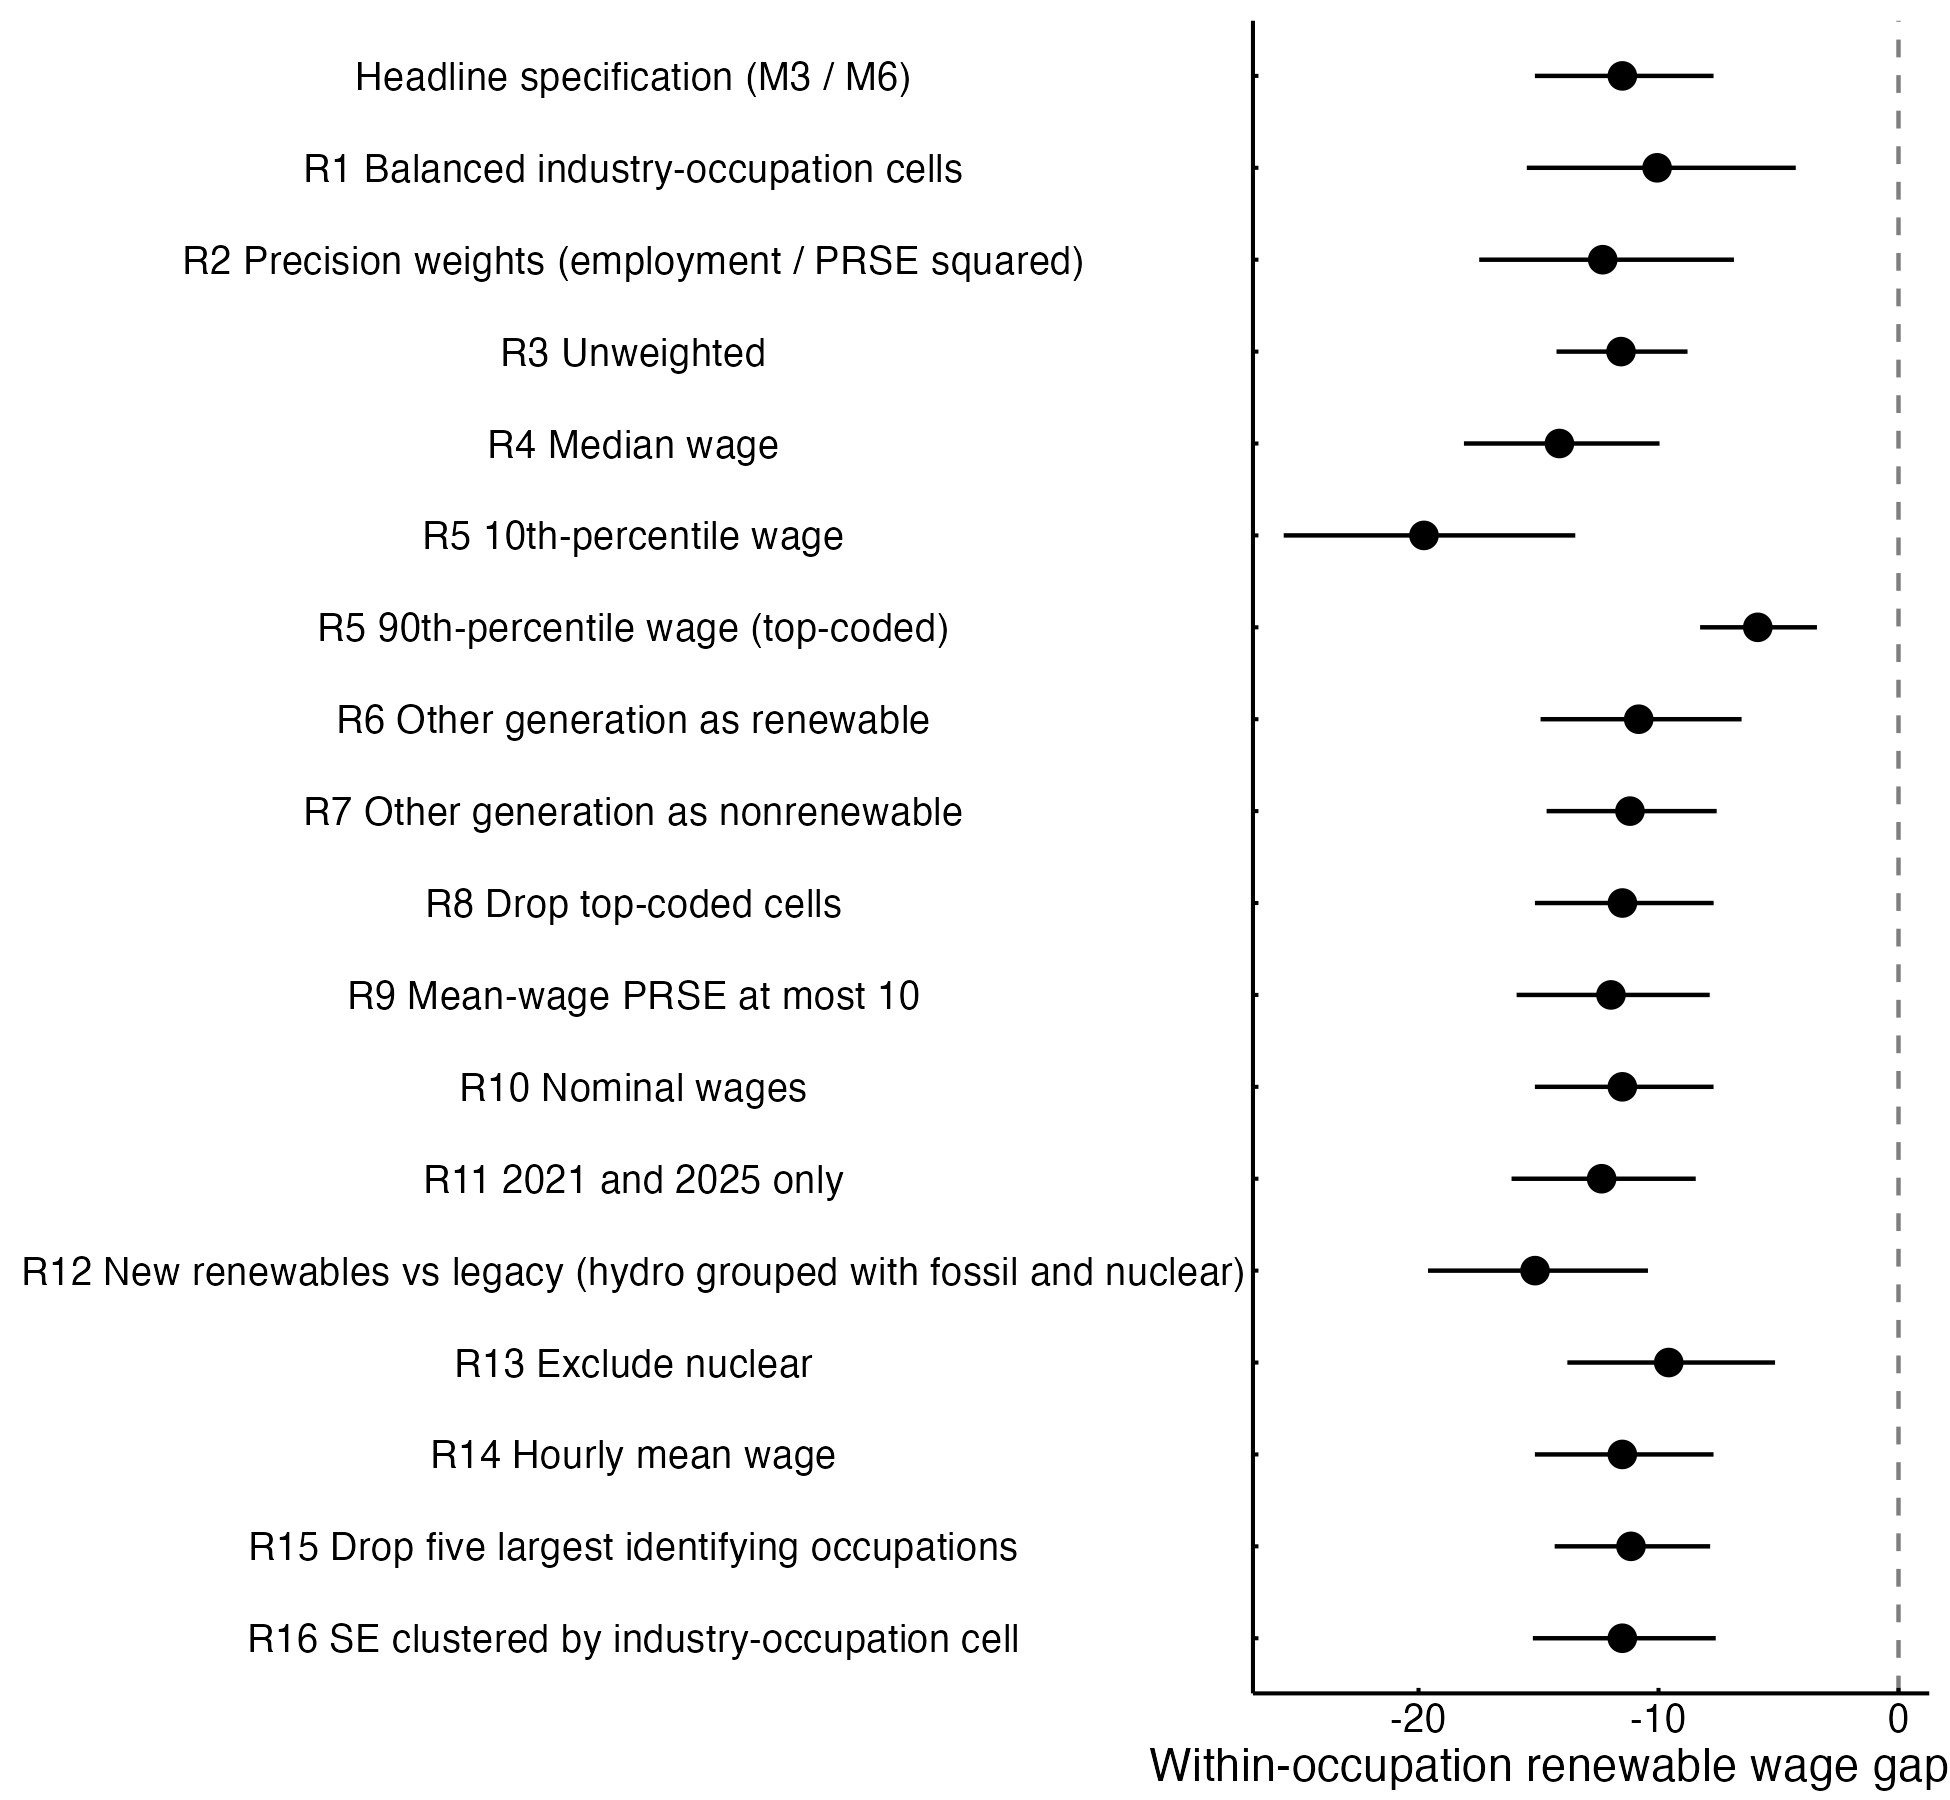
\includegraphics[width=0.85\linewidth,height=\textheight,keepaspectratio,alt={Fig. A1. Within-occupation renewable wage gap (percent) across sixteen robustness specifications; bars are 95\% confidence intervals.}]{../figures/figA1-robustness.png}
\caption{Fig. A1. Within-occupation renewable wage gap (percent) across
sixteen robustness specifications; bars are 95\% confidence intervals.}
\end{figure}

\end{document}
